\documentclass[dvipsnames, svgnames, x11names, a4paper, 11pt, oneside]{book}

\usepackage{xcolor}
% URLs and hyperlinks ---------------------------------------
\usepackage{hyperref}
\hypersetup{
	colorlinks=true,
	linkcolor=blue,
	filecolor=magenta,      
	urlcolor=blue,
}
\usepackage{xurl}
%---------------------------------------------------
\usepackage{graphicx}

\usepackage{listings}
\usepackage{color}

\definecolor{dkgreen}{rgb}{0,0.6,0}
\definecolor{gray}{rgb}{0.5,0.5,0.5}
\definecolor{mauve}{rgb}{0.58,0,0.82}

\lstset{frame=tb,
	language=vhdl,
	aboveskip=3mm,
	belowskip=3mm,
	showstringspaces=false,
	columns=flexible,
	basicstyle=\ttfamily,
	numbers=left,
	numberstyle=\small\color{gray},
	keywordstyle=\bfseries\color{Green4},
	commentstyle=\color{gray},
	stringstyle=\color{mauve},
	breaklines=true,
	breakatwhitespace=true,
	tabsize=4,
	identifierstyle=\color{black}
}

\usepackage{xepersian}
\settextfont{Yas}

\newcommand{\alu}{\lr{ALU}}

% section numbering -----------------------------------------
\setcounter{secnumdepth}{3}
\setcounter{tocdepth}{3}
%------------------------------------------------------------

\title{گزارش تمرین عملی دوم}
\author{مهدی حق‌وردی}

\begin{document}
	\maketitle
	\frontmatter
	\tableofcontents
	
	\mainmatter
		\chapter{ماژول‌‌های ساختار جمع}
			برای پیاده‌سازی عملیت جمع در این \alu از یک \lr{Half adder} یک بیتی، یک \lr{Full adder} یک بیتی استفاده شده که در کنار هم یک \lr{Four bit full adder} را تشکیل می‌دهند.
			
				\section{ماژول \lr{Half Adder}}
					\subsection{کد این ماژول}		
						\begin{latin}
							\begin{lstlisting}
library ieee;
use ieee.std_logic_1164.all;

entity half_adder is
	port (
		a, b : in std_logic;
		sum, carry : out std_logic
	);
end half_adder;

architecture arch of half_adder is
begin
	sum <= a xor b;
	carry <= a and b;
end arch;
						\end{lstlisting}
						\url{https://github.com/mahdihaghverdi/archproject/blob/main/ALU/src/half_adder/half_adder.vhdl}
						\end{latin}	
					\subsection{تست‌بنچ ۱ این ماژول}
					
						\begin{latin}
							\begin{lstlisting}
library ieee;
use ieee.std_logic_1164.all;


entity half_adder_tb is
end half_adder_tb;

architecture tb of half_adder_tb is
	signal a, b : std_logic;  -- inputs
	signal sum, carry : std_logic;  -- outputs
begin
	-- connecting testbench signals with half_adder.vhd
	UUT : entity work.half_adder port map (
			a => a,
			b => b,
			sum => sum,
			carry => carry
		);
	
	-- inputs
	-- ba
	-- 00 at 0 ns
	-- 01 at 20 ns, as b is 0 at 20 ns and a is changed to 1 at 20 ns
	-- 10 at 40 ns
	-- 11 at 60 ns
	-- 11 at 80 ns
	a <= '0', '1' after 20 ns, '0' after 40 ns, '1' after 60 ns, '1' after 80 ns;
	b <= '0', '1' after 40 ns, '1' after 60 ns;
end tb ;
							\end{lstlisting}
							\url{https://github.com/mahdihaghverdi/archproject/blob/main/ALU/src/half_adder/half_adder_tb.vhdl}
						\end{latin}	
					\subsection{تست‌بنچ ۲ این ماژول}
					
						\begin{latin}
							\begin{lstlisting}
-- half_adder_process_tb.vhd

library ieee;
use ieee.std_logic_1164.all;

entity half_adder_process_tb is
end half_adder_process_tb;

architecture tb of half_adder_process_tb is
	signal a, b : std_logic;
	signal sum, carry : std_logic;
begin
	-- connecting testbench signals with half_adder.vhd
	UUT : entity work.half_adder port map (
		a => a,
		b => b,
		sum => sum,
		carry => carry
	);

	tb1 : process
		constant period: time := 20 ns;
		begin
			a <= '0';
			b <= '0';
			wait for period;
			assert ((sum = '0') and (carry = '0'))  -- expected output
			-- error will be reported if sum or carry is not 0
			report "test failed for input combination 00" severity error;
			
			a <= '0';
			b <= '1';
			wait for period;
			assert ((sum = '1') and (carry = '0'))
			report "test failed for input combination 01" severity error;
			
			a <= '1';
			b <= '0';
			wait for period;
			assert ((sum = '1') and (carry = '0'))
			report "test failed for input combination 10" severity error;
			
			a <= '1';
			b <= '1';
			wait for period;
			assert ((sum = '0') and (carry = '1'))
			report "test failed for input combination 11" severity error;
			
			wait; -- indefinitely suspend process
	end process;
end tb;			
							\end{lstlisting}
						\url{https://github.com/mahdihaghverdi/archproject/blob/main/ALU/src/half_adder/half_adder_process_tb.vhdl}
						\end{latin}
					\subsection{خروجی \lr{simulation}}
						\begin{center}
							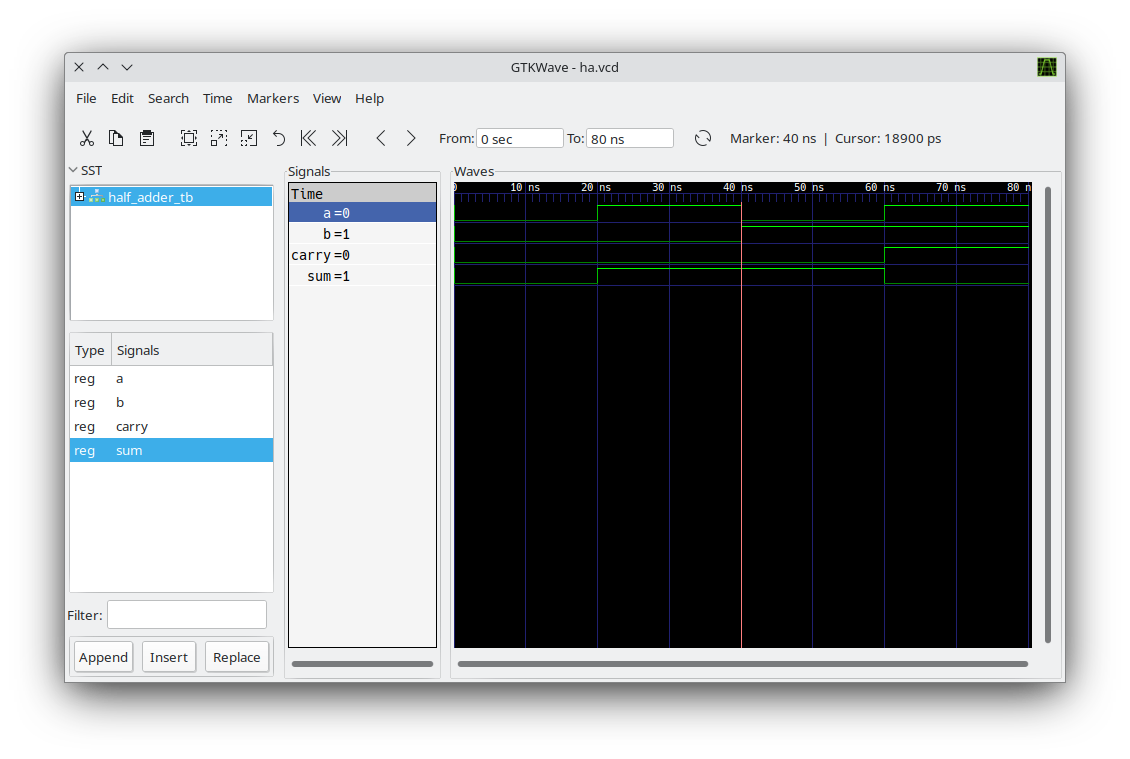
\includegraphics[width=12cm, height=9cm]{./images/half_adder_vcd}
						\end{center}
				\clearpage
				\section{ماژول \lr{Full Adder}}
					\subsection{کد این ماژول}
					
						\begin{latin}
							\begin{lstlisting}
-- one bit full adder

library ieee;
use ieee.std_logic_1164.all;

entity full_adder is
	port (
		a, b, ci : in std_logic;
		s, c : out std_logic
	);
end full_adder;


architecture arch of full_adder is
	component half_adder
		port (
			a, b : in std_logic;
			sum, carry : out std_logic
		);
	end component;

	for half_adder_0: half_adder use entity work.half_adder;
	for half_adder_1: half_adder use entity work.half_adder;
	signal asb, aab, asbco: std_logic;

begin
	half_adder_0: half_adder port map(
		-- entity-signal-name => local-signal-name
		a => a,
		b => b,
		sum => asb,
		carry => aab
	);
	half_adder_1: half_adder port map(
		a => asb,
		b => ci,
		sum => s,
		carry => asbco
	);

	c <= aab or asbco;
end arch;
							\end{lstlisting}
							\url{https://github.com/mahdihaghverdi/archproject/blob/main/ALU/src/full_adder/full_adder.vhdl}
						\end{latin}
					\subsection{تست‌‌بنچ 1 این ماژول}
					
						\begin{latin}
							\begin{lstlisting}
library ieee;
use ieee.std_logic_1164.all;

entity full_adder_tb is
end full_adder_tb;

architecture tb of full_adder_tb is
	signal a, b, ci : std_logic;  -- inputs
	signal sum, carry : std_logic;  -- outputs
begin
	-- connecting testbench signals with full_adder.vhdl
	UUT : entity work.full_adder port map (
		a => a,
		b => b,
		ci => ci,
		s => sum,
		c => carry
	);
	
	-- inputs
	-- ci ba
	--  0 00 at   0 ns
	--  0 01 at  20 ns
	--  0 10 at  40 ns
	--  0 11 at  60 ns
	--  1 00 at  80 ns
	--  1 01 at 100 ns
	--  1 10 at 120 ns
	--  1 11 at 140 ns
	--  1 11 at 160 ns
	
	a <= '0', '1' after 20 ns, '0' after 40 ns, '1' after 60 ns, '0' after 80 ns, '1' after 100 ns, '0' after 120 ns, '1' after 140 ns, '1' after 160 ns;
	b <= '0', '1' after 40 ns, '0' after 80 ns, '0' after 120 ns, '1' after 140 ns, '1' after 160 ns;
	ci <= '0', '1' after 80 ns, '1' after 120 ns, '1' after 160 ns;
end tb ;
							\end{lstlisting}
							\url{https://github.com/mahdihaghverdi/archproject/blob/main/ALU/src/full_adder/full_adder_tb.vhdl}
						\end{latin}	
					\subsection{تست‌‌بنچ 2 این ماژول}
					
						\begin{latin}
							\begin{lstlisting}
library ieee;
use ieee.std_logic_1164.all;


entity full_adder_process_tb is
end full_adder_process_tb;

architecture tb of full_adder_process_tb is
	signal a, b, ci : std_logic;  -- inputs
	signal sum, carry : std_logic;  -- outputs
begin
	-- connecting testbench signals with full_adder.vhdl
	UUT : entity work.full_adder port map (
		a => a,
		b => b,
		ci => ci,
		s => sum,
		c => carry
	);
	tb1 : process
		constant period: time := 20 ns;
		begin
		-- a b  s c
		-- 0 0  0 0
		-- 0 1  1 0
		-- 1 0  1 0
		-- 1 1  0 1
		
		a <= '0';
		b <= '0';
		ci <= '0';
		wait for period;
		assert ((sum = '0') and (carry = '0'))  -- expected output
		-- error will be reported if sum or carry is not 0
		report "test failed for input combination 000" severity error;
		
		a <= '0';
		b <= '1';
		ci <= '0';
		wait for period;
		assert ((sum = '1') and (carry = '0'))
		report "test failed for input combination 001" severity error;
		
		a <= '1';
		b <= '0';
		ci <= '0';
		wait for period;
		assert ((sum = '1') and (carry = '0'))
		report "test failed for input combination 010" severity error;
		
		a <= '1';
		b <= '1';
		ci <= '0';
		wait for period;
		assert ((sum = '0') and (carry = '1'))
		report "test failed for input combination 011" severity error;
		
		
		a <= '0';
		b <= '0';
		ci <= '1';
		wait for period;
		assert ((sum = '1') and (carry = '0'))  -- expected output
		-- error will be reported if sum or carry is not 0
		report "test failed for input combination 100" severity error;
		
		a <= '0';
		b <= '1';
		ci <= '1';
		wait for period;
		assert ((sum = '0') and (carry = '1'))
		report "test failed for input combination 101" severity error;
		
		a <= '1';
		b <= '0';
		ci <= '1';
		wait for period;
		assert ((sum = '0') and (carry = '1'))
		report "test failed for input combination 110" severity error;
		
		a <= '1';
		b <= '1';
		ci <= '1';
		wait for period;
		assert ((sum = '1') and (carry = '1'))
		report "test failed for input combination 111" severity error;
		
		
		assert false report "all tests passed." severity note;
		wait; -- indefinitely suspend process
	end process;
end tb ;
							\end{lstlisting}
						\url{https://github.com/mahdihaghverdi/archproject/blob/main/ALU/src/full_adder/full_adder_process_tb.vhdl}
						\end{latin}
					\subsection{خروجی \lr{simulation}}
						\begin{center}
							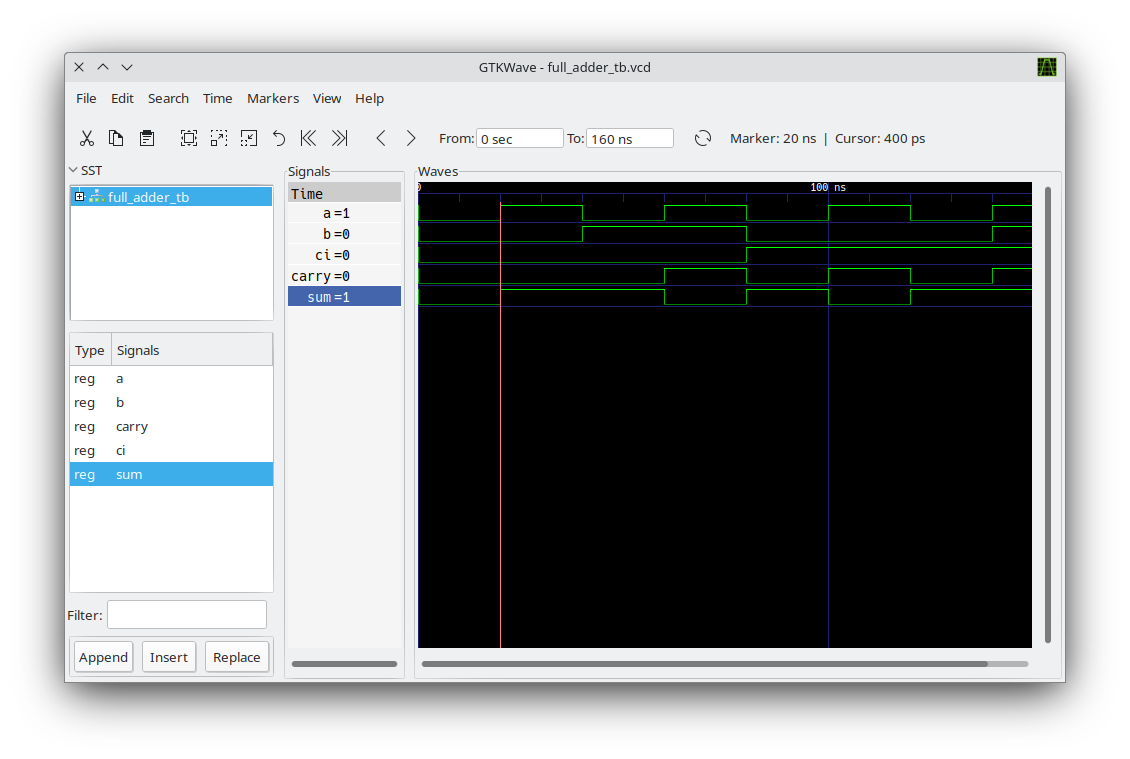
\includegraphics[width=12cm, height=8cm]{./images/full_adder_vcd_2}	
						\end{center}
						\begin{center}
							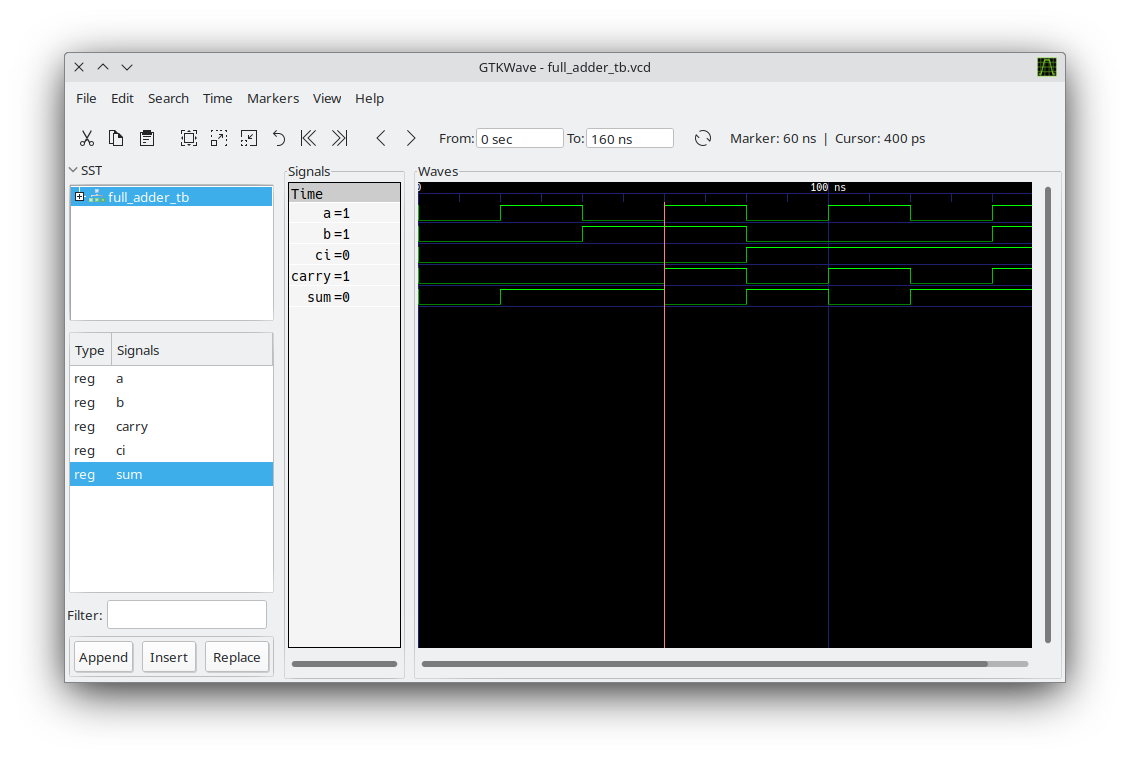
\includegraphics[width=12cm, height=9cm]{./images/full_adder_vcd_3}	
						\end{center}
						\begin{center}
							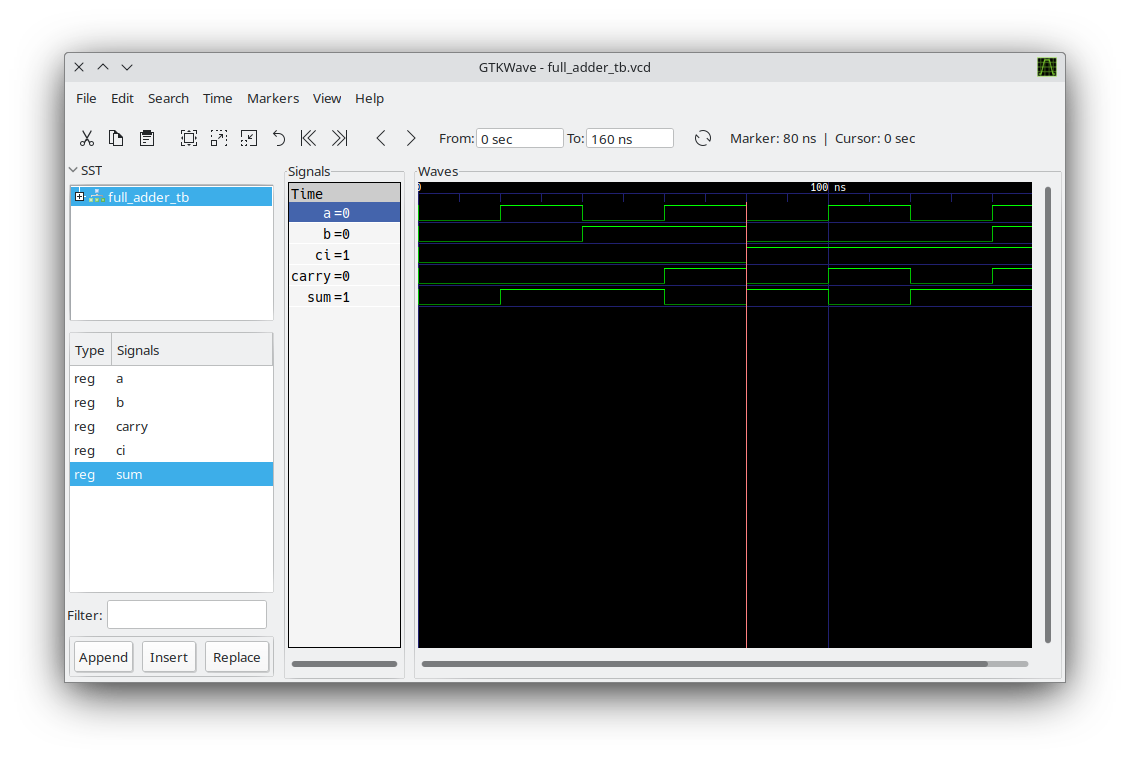
\includegraphics[width=12cm, height=9cm]{./images/full_adder_vcd_4}	
						\end{center}
				\clearpage
				\section{\lr{Four Bit Full Adder}}
					\subsection{کد این ماژول}
					\begin{latin}
						\begin{lstlisting}
library ieee;
use ieee.std_logic_1164.all;

entity FourBitFullAdder is
	port (
		input_a, input_b : in std_logic_vector (3 downto 0);
		sum : out std_logic_vector (3 downto 0);
		carry : out std_logic
	);
end FourBitFullAdder;

architecture arch of FourBitFullAdder is
	component full_adder
		port (
			a, b, ci : in std_logic;
			s, c : out std_logic
		);
	end component;
	
	for full_adder_0: full_adder use entity work.full_adder;
	for full_adder_1: full_adder use entity work.full_adder;
	for full_adder_2: full_adder use entity work.full_adder;
	for full_adder_3: full_adder use entity work.full_adder;
	
	signal carry_0_1, carry_1_2, carry_2_3 : std_logic;
begin
	full_adder_0: full_adder port map (
		a => input_a(0),
		b => input_b(0),
		ci => '0',
		s => sum(0),
		c => carry_0_1
	);
	full_adder_1: full_adder port map (
		a => input_a(1),
		b => input_b(1),
		ci => carry_0_1,
		s => sum(1),
		c => carry_1_2
	);
	full_adder_2: full_adder port map (
		a => input_a(2),
		b => input_b(2),
		ci => carry_1_2,
		s => sum(2),
		c => carry_2_3
	);
	full_adder_3: full_adder port map (
		a => input_a(3),
		b => input_b(3),
		ci => carry_2_3,
		s => sum(3),
		c => carry
	);

end arch;
						\end{lstlisting}
					\url{https://github.com/mahdihaghverdi/archproject/blob/main/ALU/src/four_bit_full_adder/four_bit_full_adder.vhdl}
					\end{latin}
				
						
					\subsection{تست‌‌بنچ این ماژول}
					
						\begin{latin}
							\begin{lstlisting}
library ieee;
use ieee.std_logic_1164.all;


entity FourBitFullAdderTB is
end FourBitFullAdderTB;

architecture tb of FourBitFullAdderTB is
	signal a, b: std_logic_vector (3 downto 0);  -- inputs
	signal sum : std_logic_vector (3 downto 0);  -- outputs
	signal carry : std_logic;

begin
	-- connecting testbench signals with 4bitfa.vhdl
	UUT : entity work.FourBitFullAdder port map (
		input_a => a,
		input_b => b,
		sum => sum,
		carry => carry
	);
	
	-- inputs and outs dec
	
	-- bb aa             c ss
	--  0  0 at  0 ns -> 0  0
	--  4  4 at 20 ns -> 0  8
	-- 12 15 at 40 ns -> 1 11
	
	-- inputs and outs bin
	-- 0000 0000 -> 0 0000
	-- 0100 0100 -> 0 1000
	-- 1100 1111 -> 1 1011
	
	a <= "0000", "0100" after 20 ns, "1111" after 40 ns, "1111" after 60 ns;
	b <= "0000", "0100" after 20 ns, "1100" after 40 ns, "1100" after 60 ns;
end tb ;
							\end{lstlisting}
							\url{https://github.com/mahdihaghverdi/archproject/blob/main/ALU/src/four_bit_full_adder/four_bit_full_adder_tb.vhdl}
						\end{latin}
					\subsection{خروجی \lr{simulation}}
						\begin{center}	
							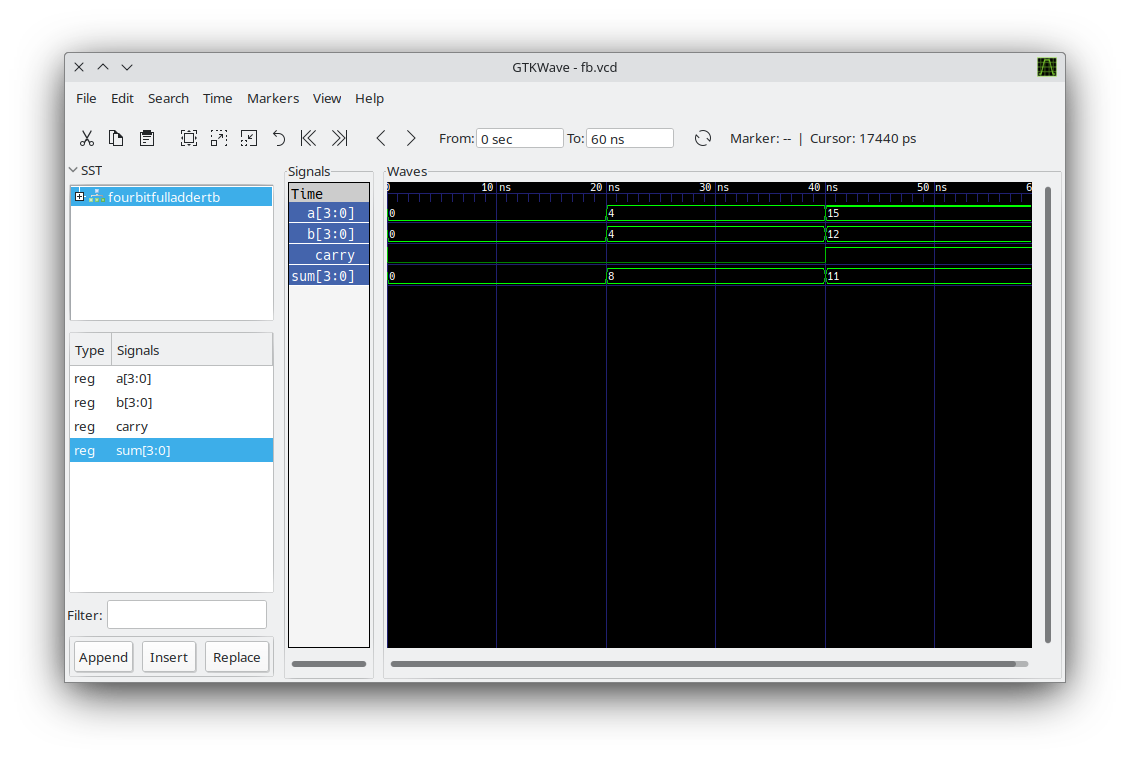
\includegraphics[width=12cm, height=9cm]{./images/four_bit_full_adder_vcd}
						\end{center}
				\section{طراحی‌ها}
					\begin{center}
						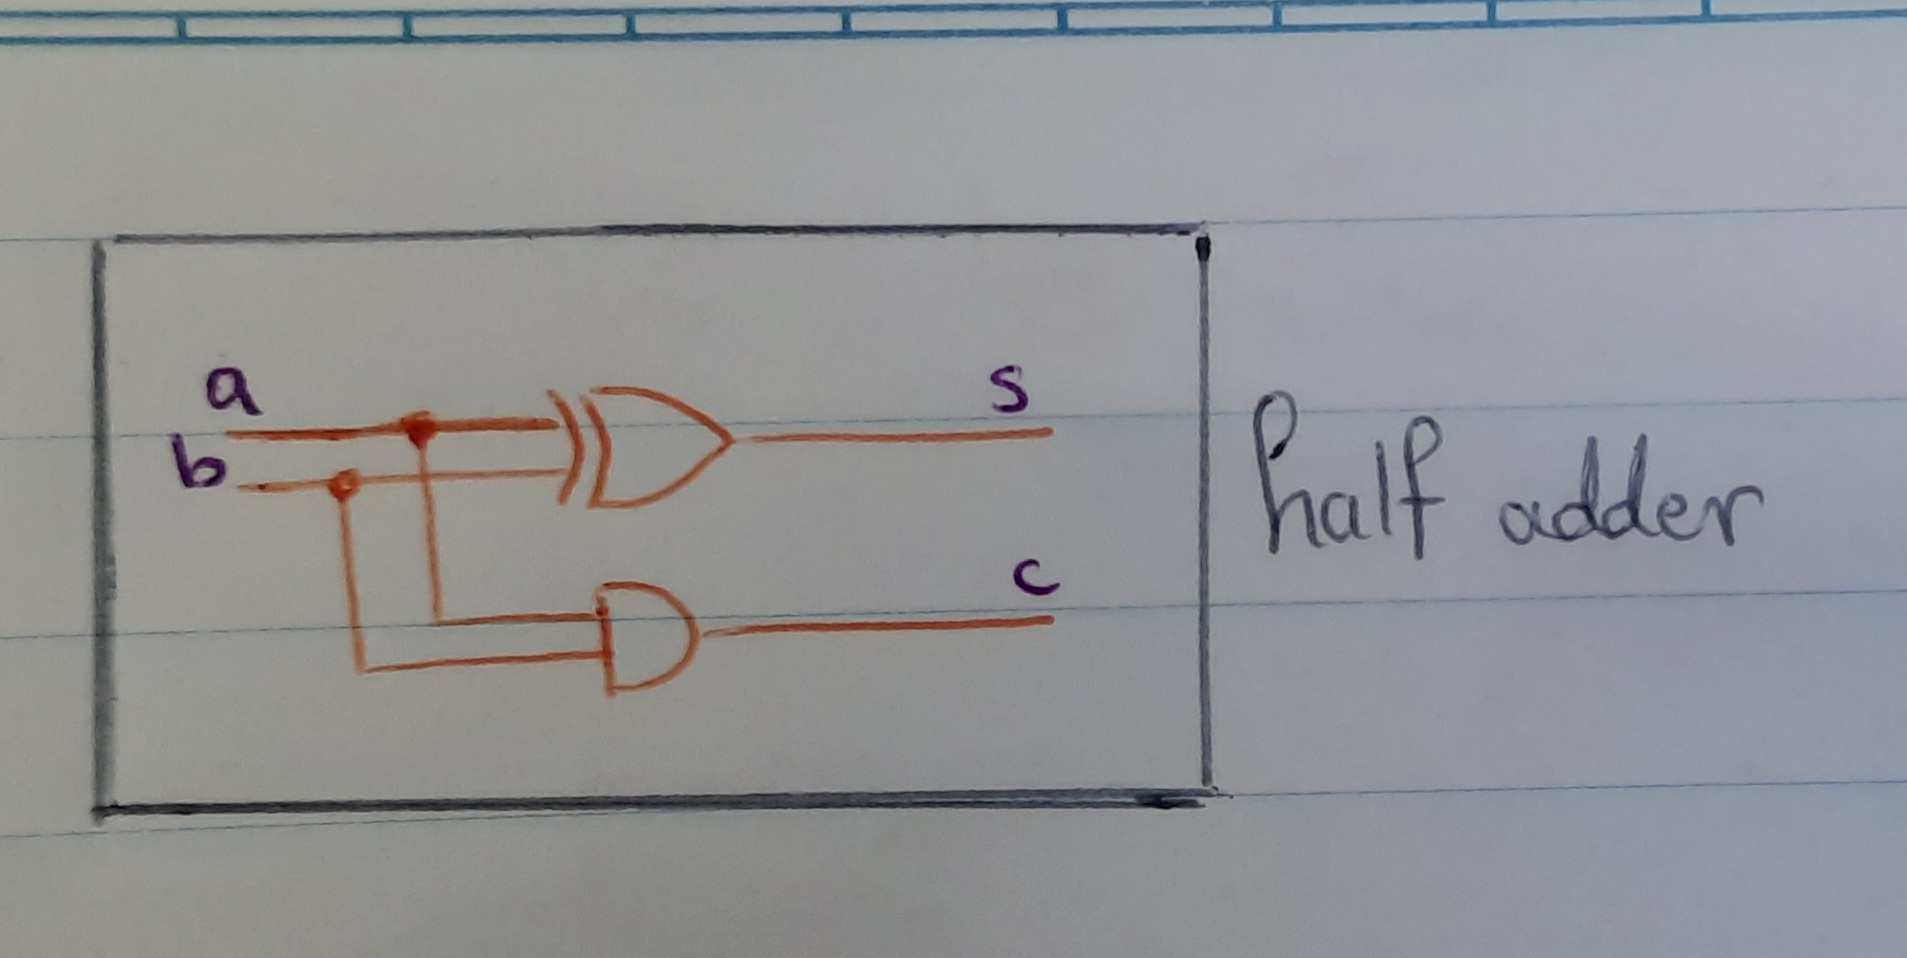
\includegraphics[width=10cm, height=8cm]{./images/adders1}
					\end{center}
				
					\begin{center}
						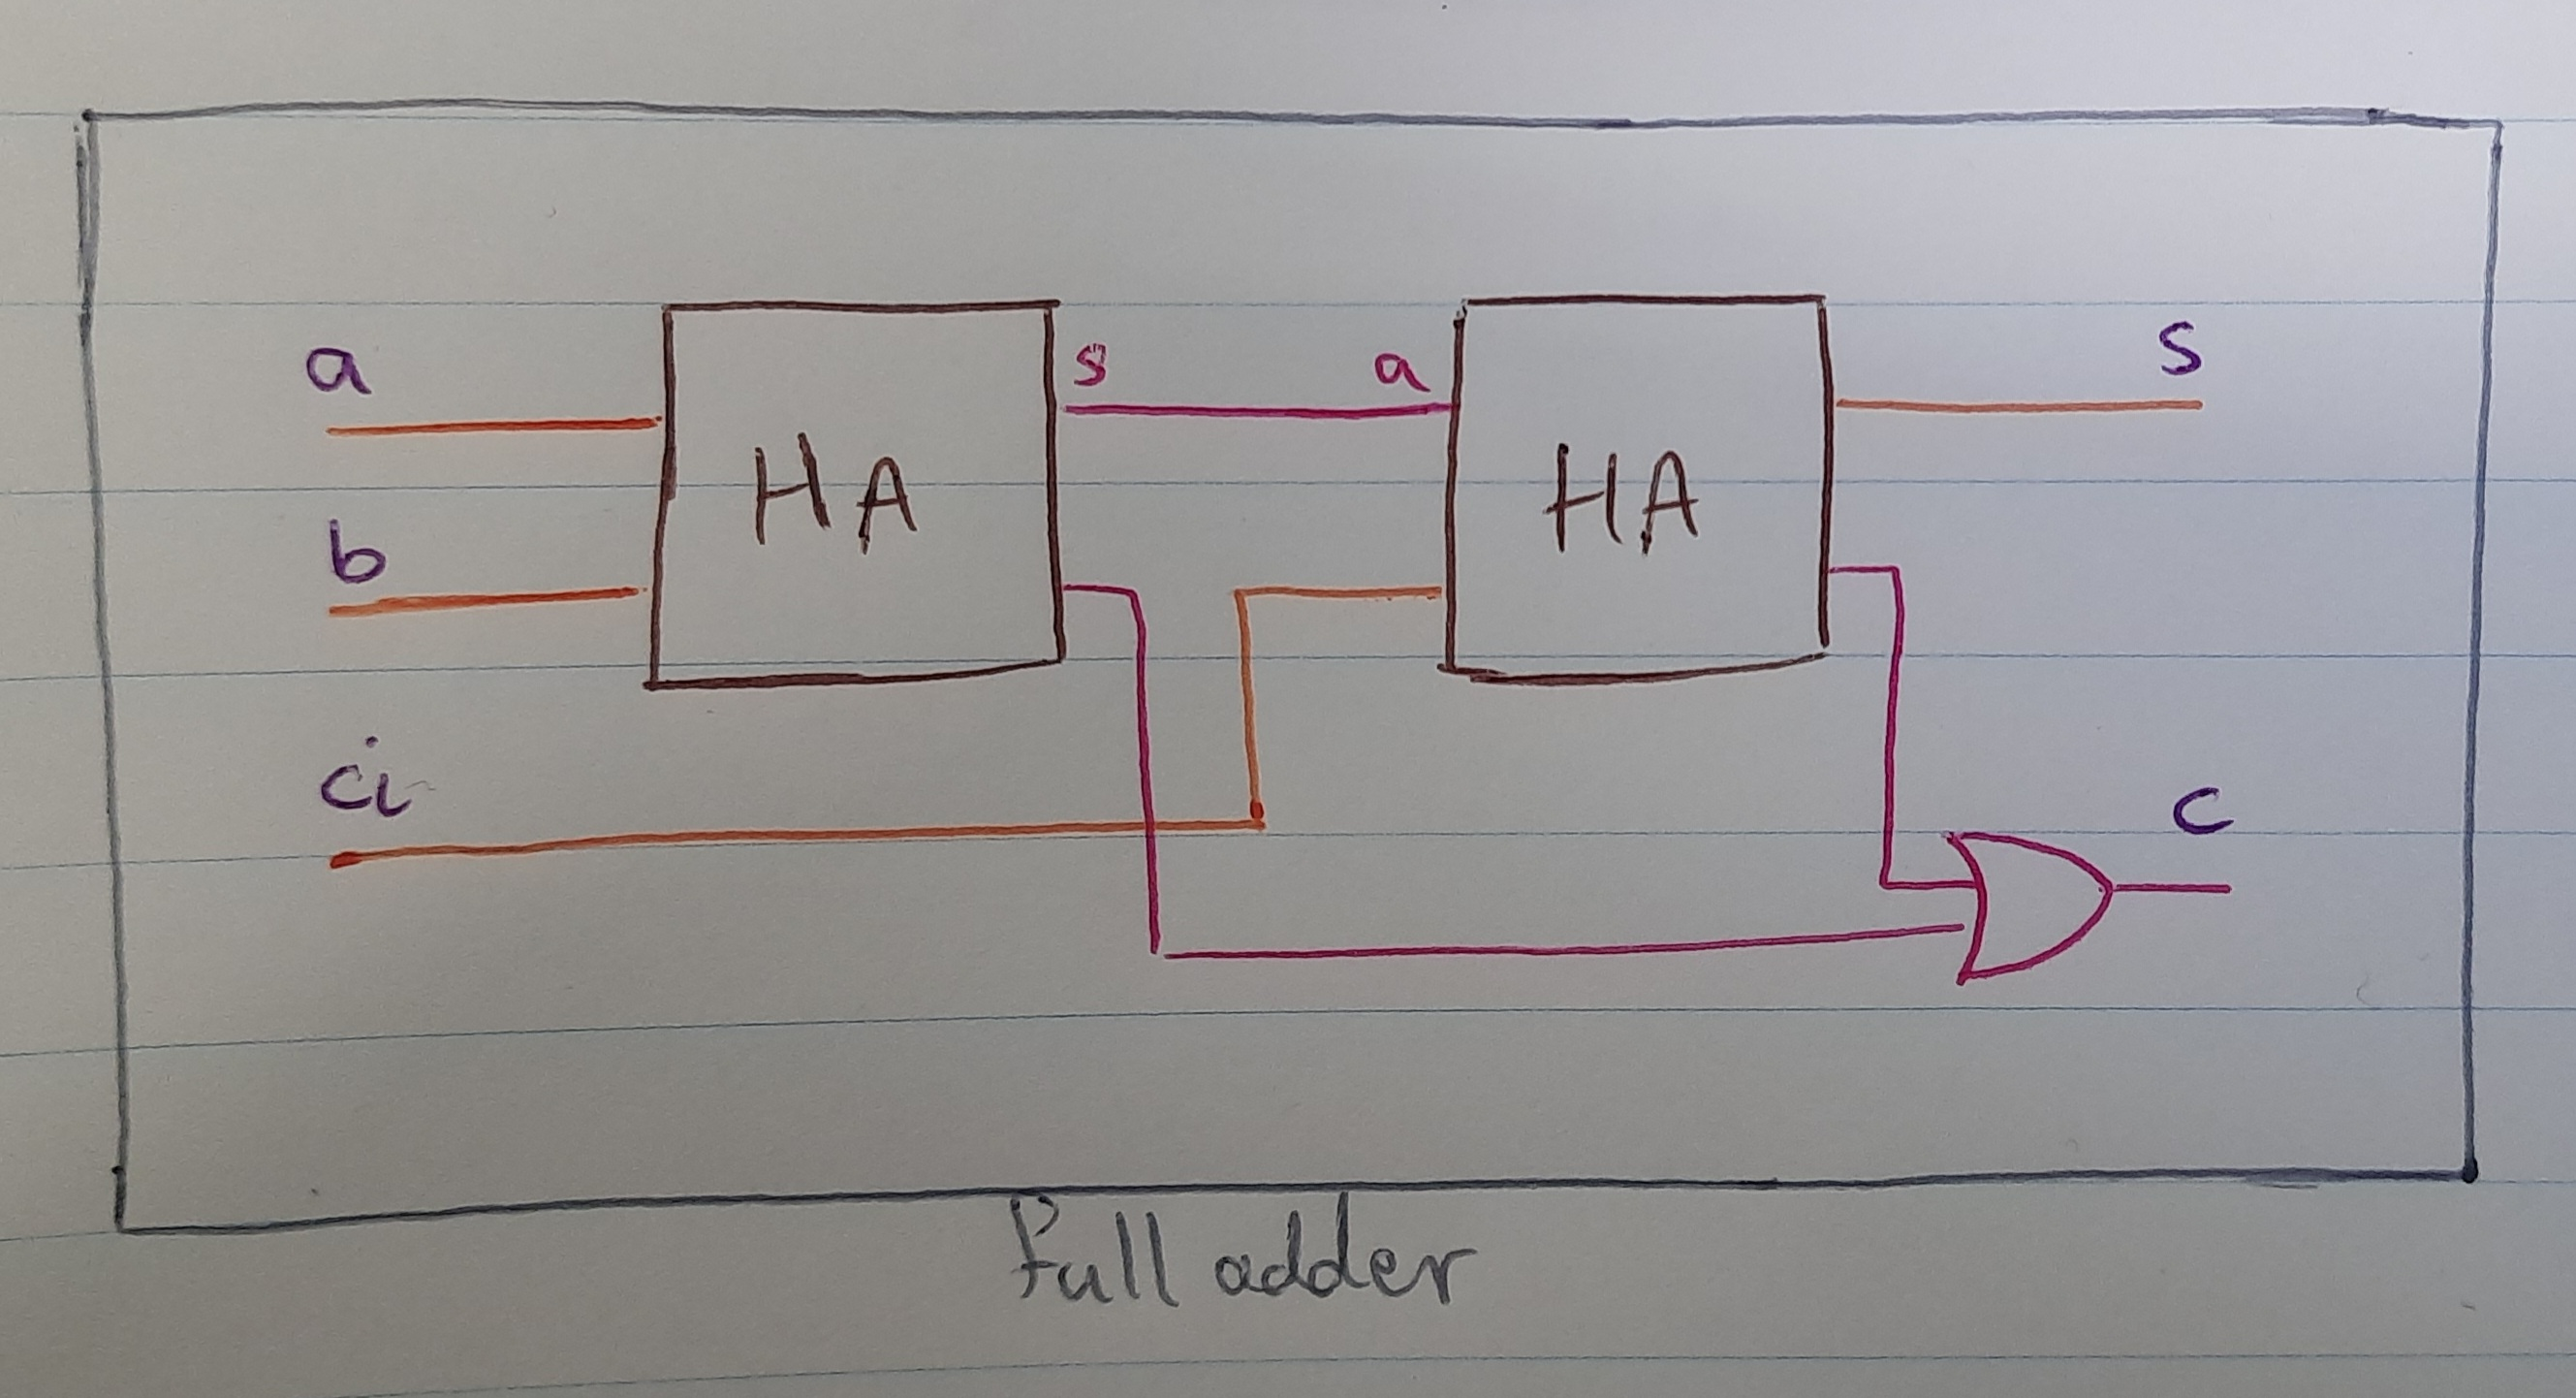
\includegraphics[width=10cm, height=8cm]{./images/adders2}
					\end{center}
					
					\begin{center}
						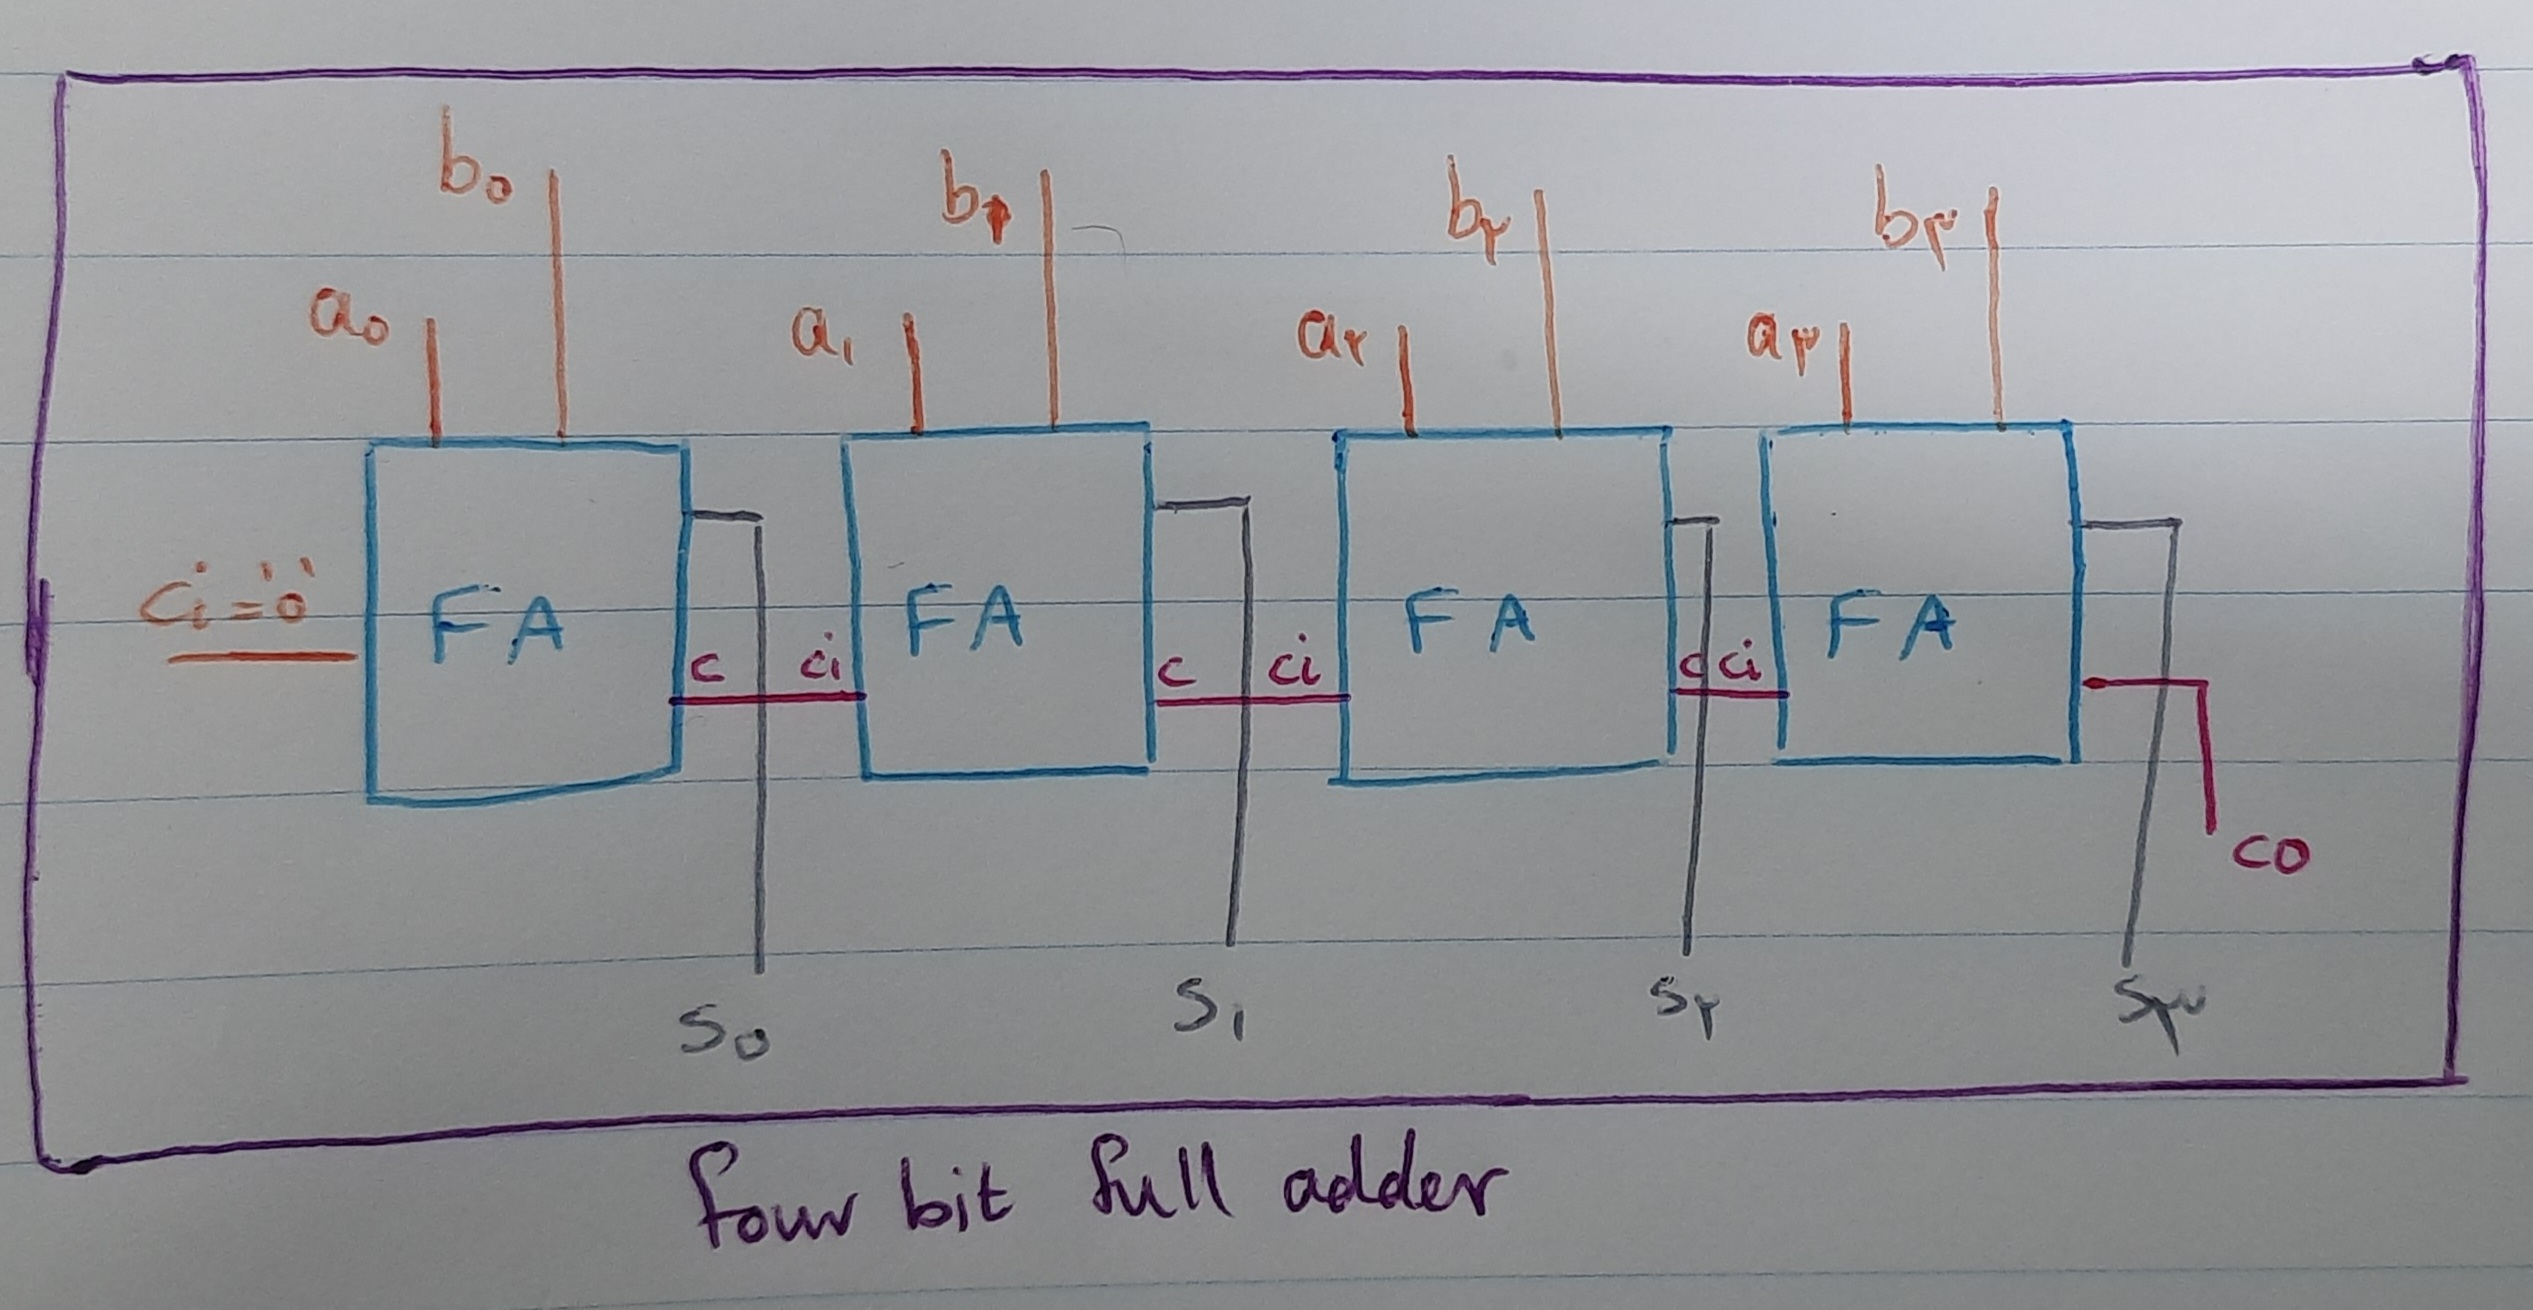
\includegraphics[width=10cm, height=8cm]{./images/adders3}
					\end{center}
				
		\clearpage
		\chapter{ماژول‌های ساختار تفریق}
			\section{ماژول \lr{Half Subber}}
				\subsection{کد این ماژول}
				
					\begin{latin}
						\begin{lstlisting}
library ieee;
use ieee.std_logic_1164.all;

entity half_subber is
	port(
		a, b: in std_logic;
		diff, borrow : out std_logic
	);
end half_subber;

architecture arch of half_subber is
begin
	diff <= a xor b;
	borrow <= not(a) and b;
end arch;			
						\end{lstlisting}
\url{https://github.com/mahdihaghverdi/archproject/blob/main/ALU/src/half_subber/half_subber.vhdl}
					\end{latin}
				\subsection{تست‌بنچ 1 ماژول}
				
					\begin{latin}
						
						\begin{lstlisting}
library ieee;
use ieee.std_logic_1164.all;


entity half_subber_tb is
end half_subber_tb;

architecture tb of half_subber_tb is
	signal a, b : std_logic;  -- inputs
	signal diff, borrow : std_logic;  -- outputs
begin
	-- connecting testbench signals with half_subber.vhdl
	UUT : entity work.half_subber port map (
		a => a,
		b => b, diff => diff,
		borrow => borrow
	);
	
	-- inputs
	-- ba             db
	-- 00 at  0 ns -> 00
	-- 01 at 20 ns -> 11
	-- 10 at 40 ns -> 10
	-- 11 at 60 ns -> 00
	-- 11 at 80 ns -> 00
	
	a <= '0', '1' after 20 ns, '0' after 40 ns, '1' after 60 ns, '1' after 80 ns;
	b <= '0', '1' after 40 ns, '1' after 60 ns;
end tb ;
						\end{lstlisting}
						\url{https://github.com/mahdihaghverdi/archproject/blob/main/ALU/src/half_subber/half_subber_tb.vhdl}
					\end{latin}
				
				\subsection{تست‌بنچ ۲ ماژول}
				
				\begin{latin}
					
					\begin{lstlisting}
-- half_subber_process_tb.vhd

library ieee;
use ieee.std_logic_1164.all;


entity half_subber_process_tb is
end half_subber_process_tb;

architecture tb of half_subber_process_tb is
	signal a, b : std_logic;
	signal diff, borrow : std_logic;
begin
	-- connecting testbench signals with half_subber.vhd
	UUT : entity work.half_subber port map (
		a => a,
		b => b,
		diff => diff,
		borrow => borrow
	);
	
	tb1 : process
		constant period: time := 20 ns;
		begin
			a <= '0';
			b <= '0';
			wait for period;
			assert ((diff = '0') and (borrow = '0'))  -- expected output
			-- error will be reported if diff or borrow is not 0
			report "test failed for input combination 00" severity error;
			
			a <= '0';
			b <= '1';
			wait for period;
			assert ((diff = '1') and (borrow = '1'))
			report "test failed for input combination 01" severity error;
			
			a <= '1';
			b <= '0';
			wait for period;
			assert ((diff = '1') and (borrow = '0'))
			report "test failed for input combination 10" severity error;
			
			a <= '1';
			b <= '1';
			wait for period;
			assert ((diff = '0') and (borrow = '0'))
			report "test failed for input combination 11" severity error;
			
			assert false report "all tests passed." severity note;
			wait; -- indefinitely suspend process
		end process;
end tb;
					\end{lstlisting}
					\url{https://github.com/mahdihaghverdi/archproject/blob/main/ALU/src/half_subber/half_subber_process_tb.vhdl}
				\end{latin}

				\subsection{خروجی \lr{simulation}}
					\begin{center}
						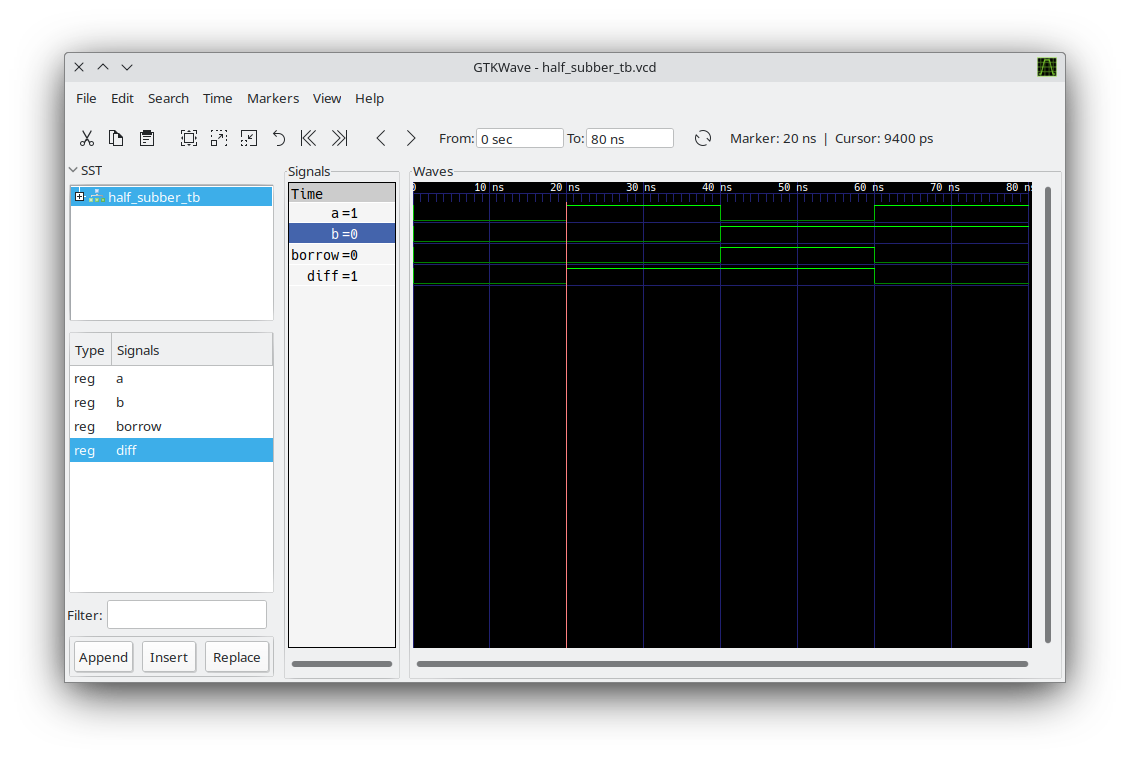
\includegraphics[width=12cm, height=8cm]{./images/half_subber_vcd_1}
					\end{center}
					
					\begin{center}
						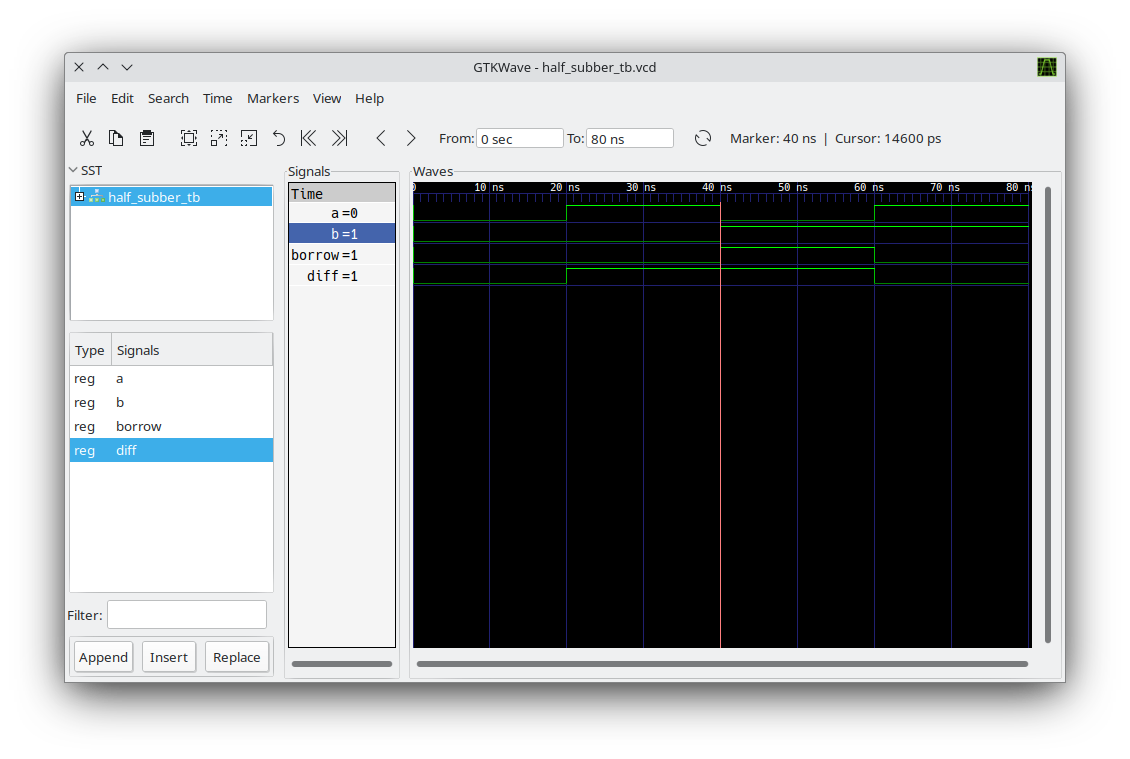
\includegraphics[width=12cm, height=9cm]{./images/half_subber_vcd_2}
					\end{center}
					\begin{center}
						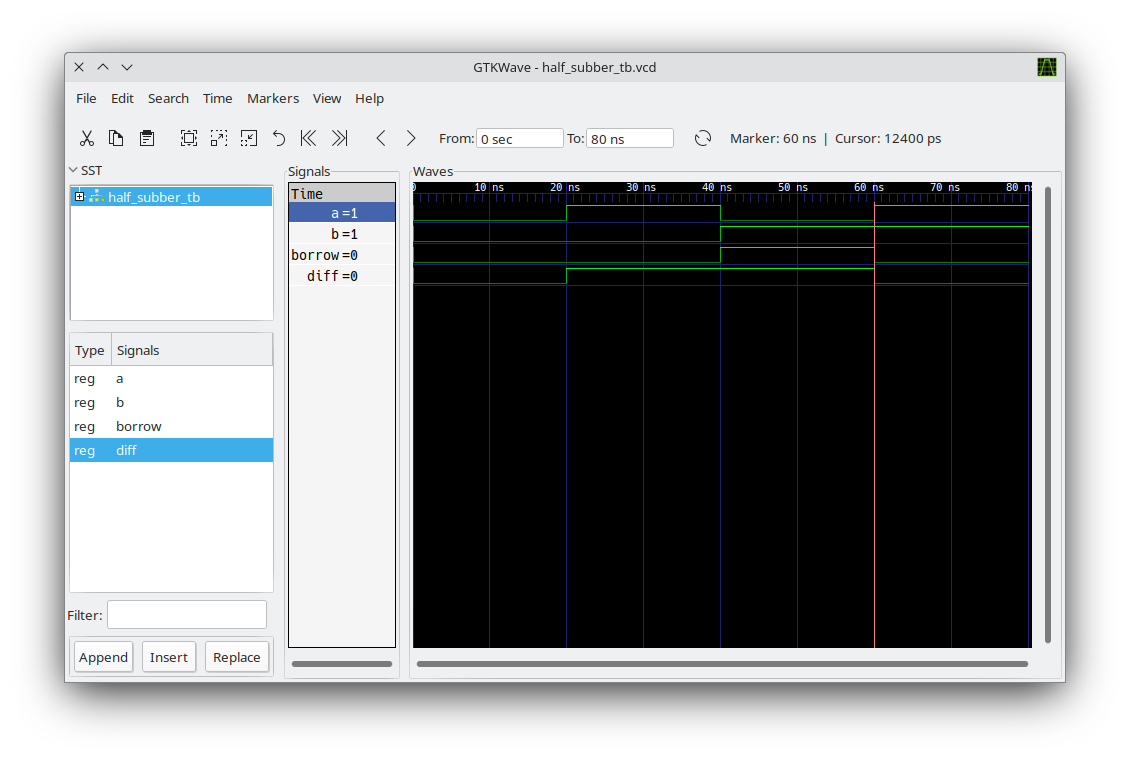
\includegraphics[width=12cm, height=9cm]{./images/half_subber_vcd_3}
					\end{center}
									
			\section{ماژول \lr{Full Subber}}
				\subsection{کد این ماژول}
					\begin{latin}
						
						\begin{lstlisting}
library ieee;
use ieee.std_logic_1164.all;

entity full_subber is
	port(
		a , b, borrow_in: in std_logic;
		diff, borrow_out : out std_logic
	);
end full_subber;

architecture arch of full_subber is
	component half_subber is
		port(
		a, b : in std_logic;
		diff, borrow : out std_logic
		);
	end component;
	
	for half_subber_0: half_subber use entity work.half_subber;
	for half_subber_1: half_subber use entity work.half_subber;
	signal adb, anab, anabi : std_logic;

begin
	half_subber_0: half_subber port map (
		a => a,
		b => b,
		diff => adb,
		borrow => anab
	);
	half_subber_1: half_subber port map (
		A => adb,
		B => borrow_in,
		diff => diff,
		borrow => anabi
	);
	
	borrow_out <= anab or anabi;
end arch;
						\end{lstlisting}
						\url{https://github.com/mahdihaghverdi/archproject/blob/main/ALU/src/full_subber/full_subber.vhdl}
					\end{latin}
				
				\subsection{تست‌بنچ ماژول}
					\begin{latin}
						
						\begin{lstlisting}
library ieee;
use ieee.std_logic_1164.all;


entity full_subber_tb is
end full_subber_tb;

architecture tb of full_subber_tb is
	signal a, b, bi : std_logic;  -- inputs
	signal diff, borrow : std_logic;  -- outputs
begin
	-- connecting testbench signals with full_subber.vhdl
	UUT : entity work.full_subber port map (
		a => a,
		b => b,
		borrow_in => bi,
		diff => diff,
		borrow_out => borrow
	);
	
	-- inputs
	-- bi ba              db
	--  0 00 at   0 ns -> 00
	--  0 01 at  20 ns -> 11
	--  1 01 at  40 ns -> 01
	--  1 11 at  60 ns -> 11
	
	bi <= '0', '1' after 40 ns, '1' after 60 ns;
	b <= '0', '1' after 60 ns;
	a <= '0', '1' after 20 ns, '1' after 60 ns;
end tb ;
						\end{lstlisting}
						\url{https://github.com/mahdihaghverdi/archproject/blob/main/ALU/src/full_subber/full_subber_tb.vhdl}
					\end{latin}
				
				\subsection{خروجی \lr{simulation}}
					\begin{center}
						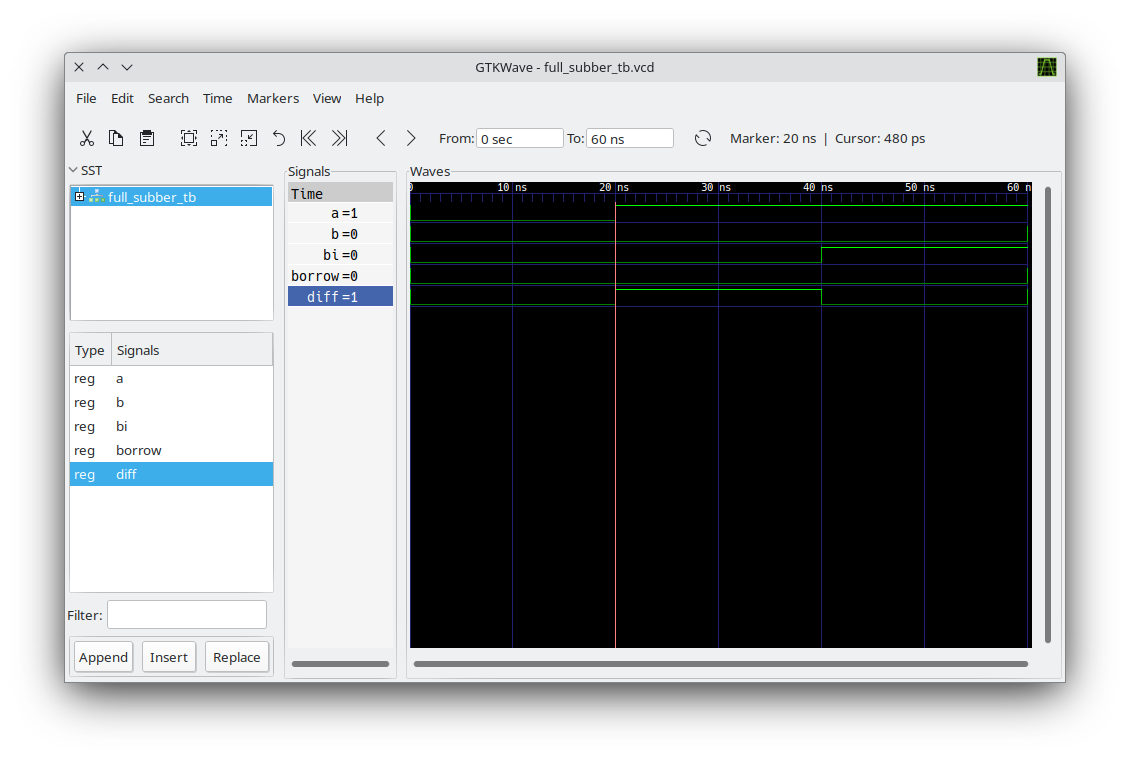
\includegraphics[width=12cm, height=8cm]{./images/full_subber_vcd_1}
					\end{center}
					
					\begin{center}
						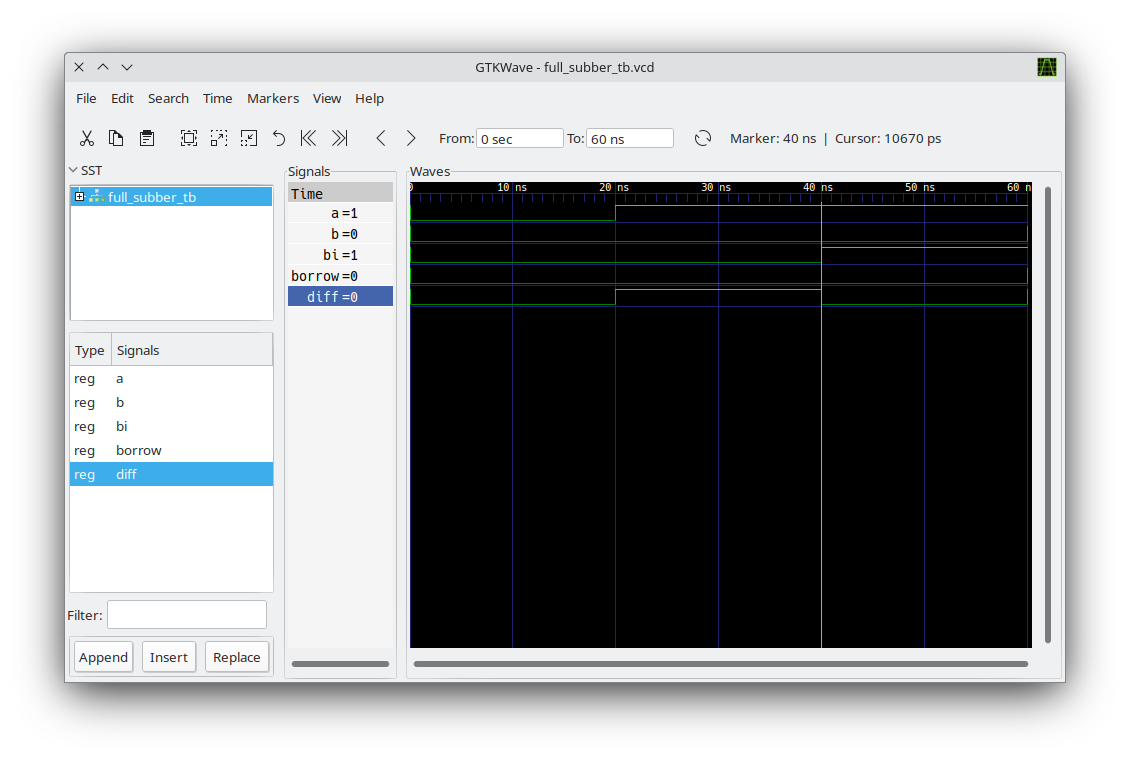
\includegraphics[width=12cm, height=9cm]{./images/full_subber_vcd_2}
					\end{center}
									
			\section{ماژول \lr{Four Bit Full Subber}}
				\subsection{کد این ماژول}
					\begin{latin}
						
						\begin{lstlisting}
library ieee;
use ieee.std_logic_1164.all;

entity FourBitFullSubber is
	port (
		input_a, input_b : in std_logic_vector (3 downto 0);
		diff : out std_logic_vector (3 downto 0);
		borrow : out std_logic
);
end FourBitFullSubber;

architecture arch of FourBitFullSubber is
	component full_subber
		port(
		a , b, borrow_in: in std_logic;
		diff, borrow_out : out std_logic
		);
	end component;
	
	for full_subber_0: full_subber use entity work.full_subber;
	for full_subber_1: full_subber use entity work.full_subber;
	for full_subber_2: full_subber use entity work.full_subber;
	for full_subber_3: full_subber use entity work.full_subber;
	
	signal borrow_0_1, borrow_1_2, borrow_2_3 : std_logic;
	begin
		full_subber_0: full_subber port map (
			a => input_a(0),
			b => input_b(0),
			borrow_in => '0',
			diff => diff(0),
			borrow_out => borrow_0_1
		);
		full_subber_1: full_subber port map (
			a => input_a(1),
			b => input_b(1),
			borrow_in => borrow_0_1,
			diff => diff(1),
			borrow_out => borrow_1_2
		);
		full_subber_2: full_subber port map (
			a => input_a(2),
			b => input_b(2),
			borrow_in => borrow_1_2,
			diff => diff(2),
			borrow_out => borrow_2_3
		);
		full_subber_3: full_subber port map (
			a => input_a(3),
			b => input_b(3),
			borrow_in => borrow_2_3,
			diff => diff(3),
			borrow_out => borrow
		);
end arch;
						\end{lstlisting}
						\url{https://github.com/mahdihaghverdi/archproject/blob/main/ALU/src/four_bit_full_subber/four_bit_full_subber.vhdl}
					\end{latin}
				\subsection{تست‌بنچ ماژول}
					\begin{latin}
						\begin{lstlisting}
library ieee;
use ieee.std_logic_1164.all;


entity FourBitFullSubberTB is
end FourBitFullSubberTB;

architecture tb of FourBitFullSubberTB is
	signal a, b: std_logic_vector (3 downto 0);  -- inputs
	signal diff : std_logic_vector (3 downto 0);  -- outputs
	signal borrow : std_logic;

begin
	-- connecting testbench signals with 4bitfa.vhdl
	UUT : entity work.FourBitFullSubber port map (
	input_a => a,
	input_b => b,
	diff => diff,
	borrow => borrow
	);
	
	-- inputs and outs dec
	
	-- b a bi              d b
	-- 0 0  0 at   0 ns -> 0 0
	-- 0 0  1 at  20 ns -> 1 1
	-- 0 1  0 at  40 ns -> 1 1
	-- 0 1  1 at  60 ns -> 0 1
	-- 1 0  0 at  80 ns -> 1 0
	-- 1 0  1 at 100 ns -> 0 0
	-- 1 1  0 at 120 ns -> 0 0
	-- 1 1  1 at 140 ns -> 1 1
	
	-- inputs and outs bin
	-- 1000 0100 -> 0 0100
	-- 1100 0100 -> 0 1000
	-- 0110 1000 -> 1 1110
	
	a <= "0000",
		  "1000" after 10 ns,
		  "1100" after 20 ns,
		  "1100" after 30 ns,
		  "0110" after 40 ns,
		  "0110" after 50 ns;
	
	b <= "0000",
	 	  "0100" after 10 ns,
	 	  "0100" after 20 ns,
	 	  "0100" after 30 ns,
	 	  "1000" after 40 ns,
	 	  "1000" after 50 ns;
end tb ;
						\end{lstlisting}
					\url{https://github.com/mahdihaghverdi/archproject/blob/main/ALU/src/four_bit_full_subber/four_bit_full_subber_tb.vhdl}
					\end{latin}
				
				\subsection{خروجی \lr{simulation}}
					\begin{center}
						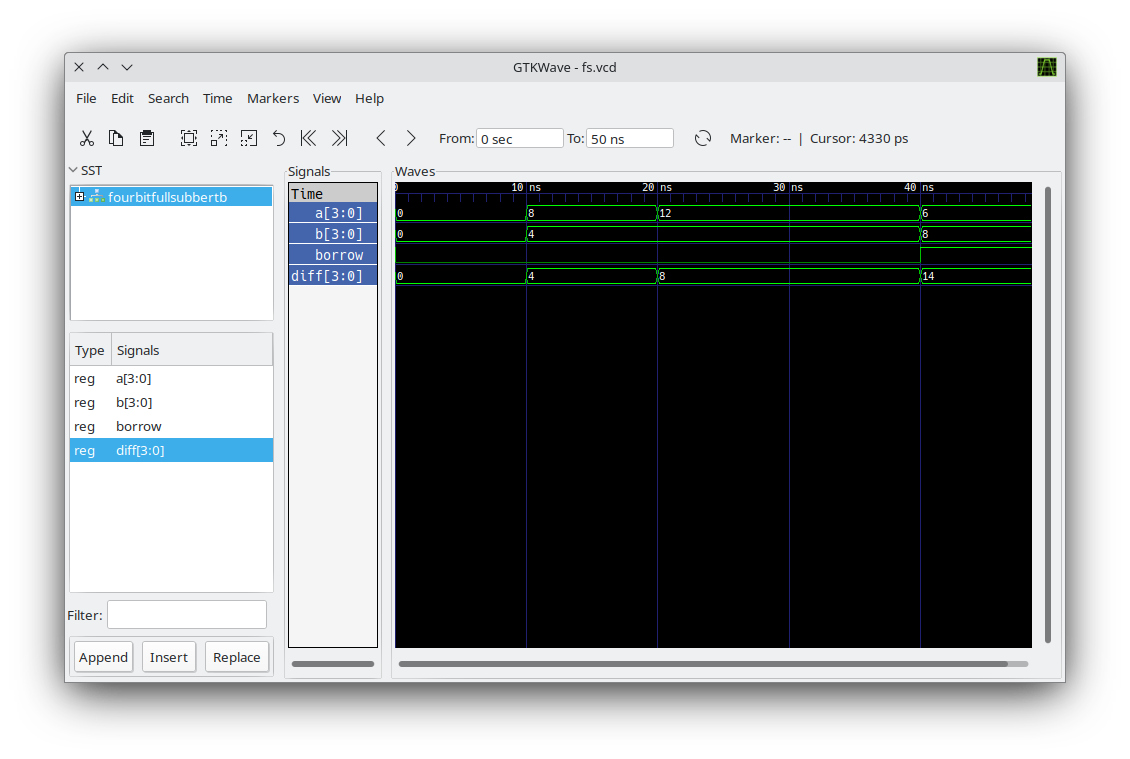
\includegraphics[width=12cm, height=9cm]{./images/four_bit_full_subber_vcd}
					\end{center}
										
			\section{طراحی‌ها}
					\begin{center}
						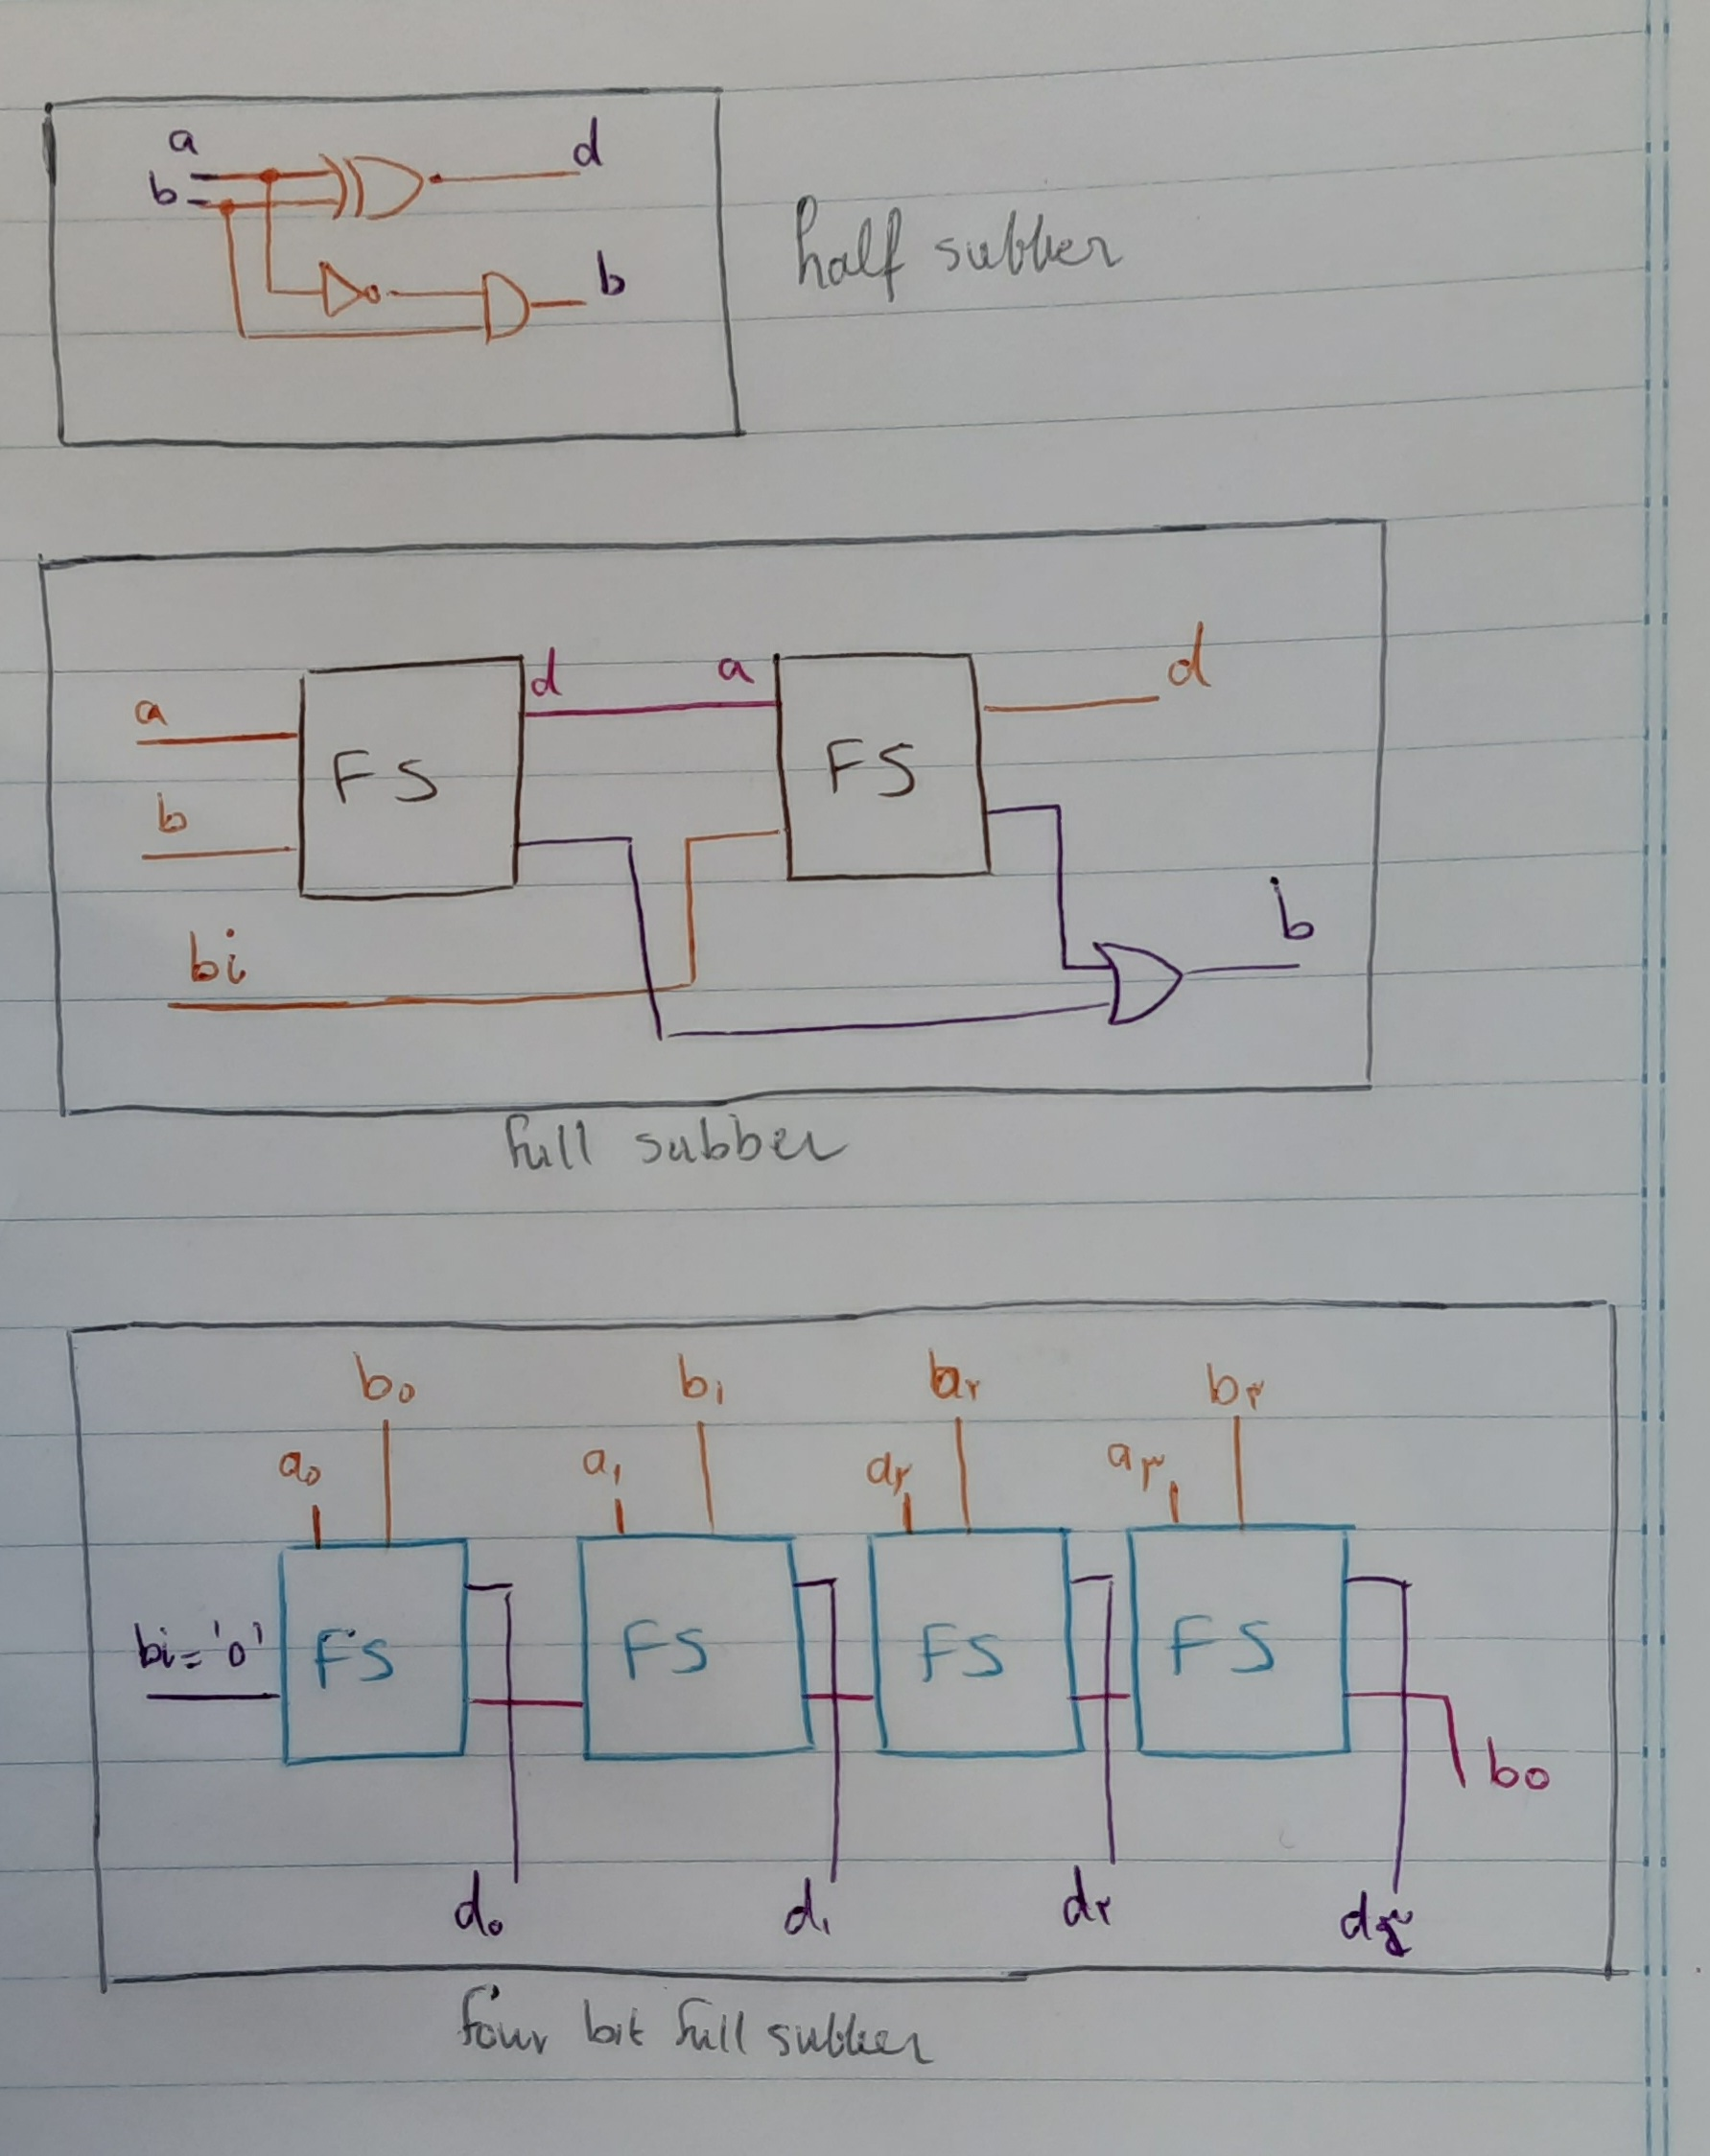
\includegraphics[width=12cm, height=18cm]{./images/subbers}
					\end{center}
				
		\clearpage			
		\chapter{ماژول‌های ساختار ضرب}
			\section{ماژول \lr{Four Bit Multiplier}}
				\subsection{کد این ماژول}
					\begin{latin}
						
						\begin{lstlisting}
library ieee;
use ieee.std_logic_1164.all;

entity FourBitMultiplier is
	port (
		input_a, input_b : in std_logic_vector (3 downto 0);
		output: out std_logic_vector (7 downto 0)
	);
end FourBitMultiplier;

architecture arch of FourBitMultiplier is
	component FourBitFullAdder
		port (
		input_a, input_b : in std_logic_vector (3 downto 0);
		sum : out std_logic_vector (3 downto 0);
		carry : out std_logic
		);
	end component;
	
	for four_bit_full_adder_0: FourBitFullAdder use entity work.FourBitFullAdder;
	for four_bit_full_adder_1: FourBitFullAdder use entity work.FourBitFullAdder;
	for four_bit_full_adder_2: FourBitFullAdder use entity work.FourBitFullAdder;
	
	signal a0b1, a0b2, a0b3 : std_logic;
	signal input_a_0, input_b_0, input_a_1, input_b_1, input_a_2, input_b_2 : std_logic_vector (3 downto 0);
	signal a1b0, a1b1, a1b2, a1b3 : std_logic;
	signal a2b0, a2b1, a2b2, a2b3 : std_logic;
	signal a3b0, a3b1, a3b2, a3b3 : std_logic;
	signal sum0, sum1, sum2 : std_logic_vector (3 downto 0);
	signal carry_0_1, carry_1_2, carry_2_3 : std_logic;
	
	begin
		a0b1 <= input_a(0) and input_b(1);
		a0b2 <= input_a(0) and input_b(2);
		a0b3 <= input_a(0) and input_b(3);
		input_a_0 <= ('0', a0b3, a0b2, a0b1);
		input_b_0 <= (a1b3, a1b2, a1b1, a1b0);
	
		a1b0 <= input_a(1) and input_b(0);
		a1b1 <= input_a(1) and input_b(1);
		a1b2 <= input_a(1) and input_b(2);
		a1b3 <= input_a(1) and input_b(3);
	
		four_bit_full_adder_0: FourBitFullAdder port map (
			input_a => input_a_0,
			input_b => input_b_0,
			sum => sum0,
			carry => carry_0_1
		);
		a2b0 <= input_a(2) and input_b(0);
		a2b1 <= input_a(2) and input_b(1);
		a2b2 <= input_a(2) and input_b(2);
		a2b3 <= input_a(2) and input_b(3);
		
		input_a_1 <= (carry_0_1, sum0(3), sum0(2), sum0(1));
		input_b_1 <= (a2b3, a2b2, a2b1, a2b0);
		
		four_bit_full_adder_1: FourBitFullAdder port map (
			input_a => input_a_1,
			input_b => input_b_1,
			sum => sum1,
			carry => carry_1_2
		);
	
		a3b0 <= input_a(3) and input_b(0);
		a3b1 <= input_a(3) and input_b(1);
		a3b2 <= input_a(3) and input_b(2);
		a3b3 <= input_a(3) and input_b(3);
		
		input_a_2 <= (carry_1_2, sum1(3), sum1(2), sum1(1));
		input_b_2 <= (a3b3, a3b2, a3b1, a3b0);
		four_bit_full_adder_2: FourBitFullAdder port map (
			input_a => input_a_2,
			input_b => input_b_2,
			sum => sum2,
			carry => carry_2_3
		);
		output <= (
			carry_2_3,
			sum2(3), sum2(2), sum2(1), sum2(0),
			sum1(0),
			sum0(0),
			input_a(0) and input_b(0)
		);
end arch;
						\end{lstlisting}
						\url{https://github.com/mahdihaghverdi/archproject/blob/main/ALU/src/four_bit_multiplier/four_bit_multiplier.vhdl}
					\end{latin}
				\subsection{تست‌بنچ این ماژول}
					\begin{latin}
						
						\begin{lstlisting}
library ieee;
use ieee.std_logic_1164.all;


entity FourBitMultiplierTB is
end FourBitMultiplierTB;

architecture tb of FourBitMultiplierTB is
	signal a, b: std_logic_vector (3 downto 0);  -- inputs
	signal output : std_logic_vector (7 downto 0);  -- outputs

begin
	-- connecting testbench signals with 4bitfa.vhdl
	UUT : entity work.FourBitMultiplier port map (
		input_a => a,
		input_b => b,
		output => output
	);
	
	-- bbbb aaaa    oooooooo
	-- 1101 1011 -> 10001111
	-- 1001 0101 -> 00101101
	-- 1010 1110 -> 10001100
	
	a <= "0000", "1011" after 20 ns, "0101" after 40 ns, "1110" after 60 ns, "1110" after 80 ns;
	b <= "0000", "1101" after 20 ns, "1001" after 40 ns, "1010" after 60 ns, "1010" after 80 ns;
end tb ;
						\end{lstlisting}
						\url{https://github.com/mahdihaghverdi/archproject/blob/main/ALU/src/four_bit_multiplier/four_bit_multplier_tb.vhdl}
					\end{latin}
				\subsection{خروجی \lr{simulation}}
					\begin{center}
						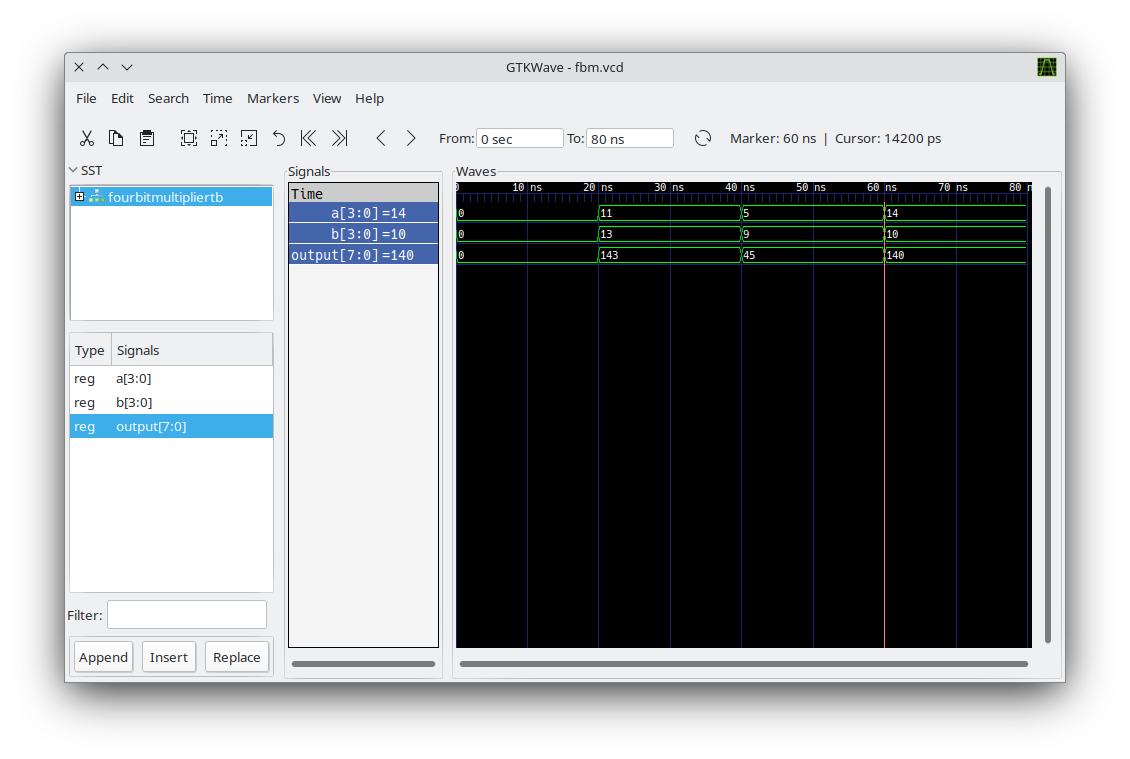
\includegraphics[width=12cm, height=9cm]{./images/four_bit_mul_vcd}
					\end{center}
				
			\section{طراحی‌ها}
				\begin{center}
					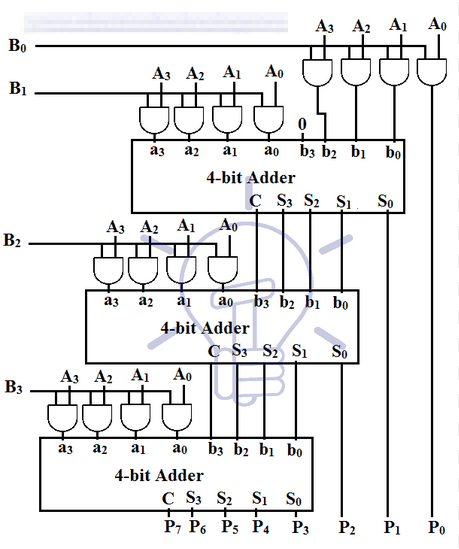
\includegraphics[width=12cm, height=15cm]{./images/mul}
				\end{center}
		
		\clearpage
		\chapter{ماژول مالتی پلکسر}
			\section{ماژول \lr{mux4x1}}
				\subsection{کد این ماژول}
					\begin{latin}
						\begin{lstlisting}
library ieee;
use ieee.std_logic_1164.all;

entity mux4x1 is
	port (
		i0, i1, i2, i3 : in std_logic_vector (7 downto 0);
		sel : in std_logic_vector (1 downto 0);
		output: out std_logic_vector (7 downto 0)
	);
end mux4x1;

architecture arch of mux4x1 is
	begin
	with sel select output <=
		i0 when "00",
		i1 when "01",
		i2 when "10",
		i3 when others;
end arch;
						\end{lstlisting}
						\url{https://github.com/mahdihaghverdi/archproject/blob/main/ALU/src/mux4x1/mux4x1.vhdl}
					\end{latin}
				
				\subsection{تست‌بنچ این ماژول}
					\begin{latin}
						
						\begin{lstlisting}
library ieee;
use ieee.std_logic_1164.all;

entity mux4x1_tb is
end mux4x1_tb;

architecture arch of mux4x1_tb is
	signal i0, i1, i2, i3, output : std_logic_vector (7 downto 0);
	signal sel : std_logic_vector (1 downto 0);
begin
	UUT : entity work.mux4x1 port map (
		i0 => i0,
		i1 => i1,
		i2 => i2,
		i3 => i3,
		sel => sel,
		output => output
	);
	
	
	-- i3333333 i2222222 i1111111 i0000000 sel   oooooooo
	-- 00001010 00000011 00000101 00000010 00    00000010
	-- 00001010 00000011 00000101 00000010 01    00000101
	-- 00001010 00000011 00000101 00000010 10    00000011
	-- 00001010 00000011 00000101 00000010 11    00001010
	
	i0 <= "00000000", "00000010" after 20 ns, "00000010" after 40 ns, "00000010" after 60 ns, "00000010" after 80 ns;
	i1 <= "00000000", "00000101" after 20 ns, "00000101" after 40 ns, "00000101" after 60 ns, "00000101" after 80 ns;
	i2 <= "00000000", "00000011" after 20 ns, "00000011" after 40 ns, "00000011" after 60 ns, "00000011" after 80 ns;
	i3 <= "00000000", "00001010" after 20 ns, "00001010" after 40 ns, "00001010" after 60 ns, "00001010" after 80 ns;
	sel <=  "00", "00" after 20 ns, "01" after 40 ns, "10" after 60 ns, "11" after 80 ns, "11" after 100 ns;

end arch;
						\end{lstlisting}
						\url{https://github.com/mahdihaghverdi/archproject/blob/main/ALU/src/mux4x1/mux4x1_tb.vhdl}
					\end{latin}
				
				\subsection{خروجی \lr{simulation}}
					\begin{center}
						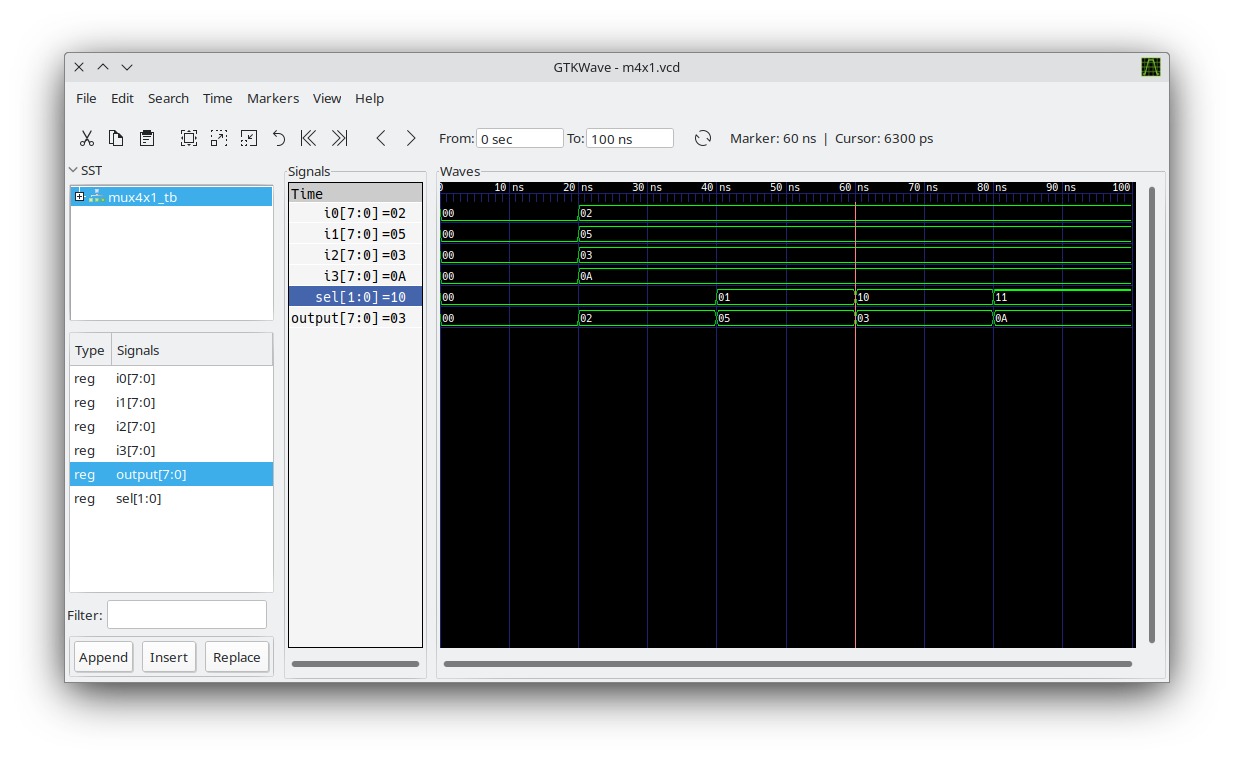
\includegraphics[width=12cm, height=9cm]{./images/mux_vcd}
					\end{center}
		\clearpage
		\chapter{ماژول \alu}
			\section{ماژول \alu}
				\subsection{کد این ماژول}
					\begin{latin}
						
						\begin{lstlisting}
library ieee;
use ieee.std_logic_1164.all;

entity alu is
port (
alu_input_a, alu_input_b: in std_logic_vector (3 downto 0);
alu_out                 : out std_logic_vector (7 downto 0);
alu_carry_borrow_out    : out std_logic;
alu_select              : in std_logic_vector (1 downto 0)
);
end alu;

architecture arch of alu is
	-- we need a mux, four_bit_full_adder/subber/multiplier
	-- 00 -> full_adder
	-- 01 -> full_subber
	-- 10 -> full_multiplier
	-- 11 -> all one :)
	
	component mux4x1
		port (
			i0, i1, i2, i3: in std_logic_vector (3 downto 0);
			sel           : in std_logic_vector (1 downto 0);
			output        : out std_logic_vector (3 downto 0)
		);
	end component;
	
	component FourBitFullAdder
		port (
			input_a, input_b: in std_logic_vector (3 downto 0);
			sum             : out std_logic_vector (3 downto 0);
			carry           : out std_logic
		);
	end component;
	
	component FourBitFullSubber
		port (
			input_a, input_b: in std_logic_vector (3 downto 0);
			diff            : out std_logic_vector (3 downto 0);
			borrow          : out std_logic
		);
	end component;
	
	component FourBitMultiplier
		port (
			input_a, input_b: in std_logic_vector (3 downto 0);
			output          : out std_logic_vector (7 downto 0)
		);
	end component;
	
	signal full_adder_to_i0_t, full_subber_to_i1_t : std_logic_vector(3 downto 0);
	signal before_alu_out : std_logic_vector(3 downto 0);
	signal multiplier_to_i2, full_adder_to_i0, full_subber_to_i1 : std_logic_vector (7 downto 0);
	signal after_alu_out : std_logic_vector (7 downto 0);
	begin
	
	
	inner_full_adder  : entity work.FourBitFullAdder port map (
		input_a => alu_input_a,
		input_b => alu_input_b,
		sum => full_adder_to_i0_t,
		carry => alu_carry_borrow_out
	);
	full_adder_to_i0 <= "0000" & full_adder_to_i0_t;
	
	inner_full_subber : entity work.FourBitFullSubber port map (
		input_a => alu_input_a,
		input_b => alu_input_b,
		diff => full_subber_to_i1_t,
		borrow => alu_carry_borrow_out
		);
	full_subber_to_i1 <= "0000" & full_subber_to_i1_t;
	
	inner_multiplier  : entity work.FourBitMultiplier port map (
		input_a => alu_input_a,
		input_b => alu_input_b,
		output => multiplier_to_i2
	);
	
	inner_mux : entity work.mux4x1 port map (
		i0 => full_adder_to_i0,
		i1 => full_subber_to_i1,
		i2 => multiplier_to_i2,
		i3 => "11111111",
		sel => alu_select,
		output => alu_out
	);
end arch;
						\end{lstlisting}
						\url{https://github.com/mahdihaghverdi/archproject/blob/main/ALU/src/alu.vhdl}
					\end{latin}
				
				\subsection{تست‌بنچ این ماژول}
				\begin{latin}
					
					\begin{lstlisting}
library ieee;
use ieee.std_logic_1164.all;

--  A testbench has no ports.
entity alu_tb is
end alu_tb;

architecture tb of alu_tb is
	signal input_a, input_b : std_logic_vector (3 downto 0);
	signal output           : std_logic_vector (7 downto 0);
	signal carry_borrow_out : std_logic;
	signal sel              : std_logic_vector (1 downto 0);

begin
	UUT : entity work.alu port map (
		alu_input_a => input_a,
		alu_input_b => input_b,
		alu_out => output,
		alu_carry_borrow_out => carry_borrow_out,
		alu_select => sel
	);
	
	-- aaaa bbbb ss ++++ ---- ******** ````
	-- 0000 0000 00 0000
	-- 0000 0000 01      0000
	-- 0000 0000 10           00000000
	-- 0000 0000 10                    1111
	
	-- 0100 0010 00 0110
	-- 0100 0010 01      0010
	-- 0100 0010 10           00001000
	-- 0100 0010 11                    1111
	
	input_a <= "0000", "0100" after 20 ns;
	input_b <= "0000", "0010" after 20 ns;
	sel <= "00", "00" after 20 ns, "01" after 40 ns, "10" after 60 ns, "11" after 80 ns, "11" after 100 ns;
end tb;
					\end{lstlisting}
					\url{https://github.com/mahdihaghverdi/archproject/blob/main/ALU/src/alu_tb.vhdl}
				\end{latin}

				\subsection{خروجی \lr{simulation}}
					\begin{center}
						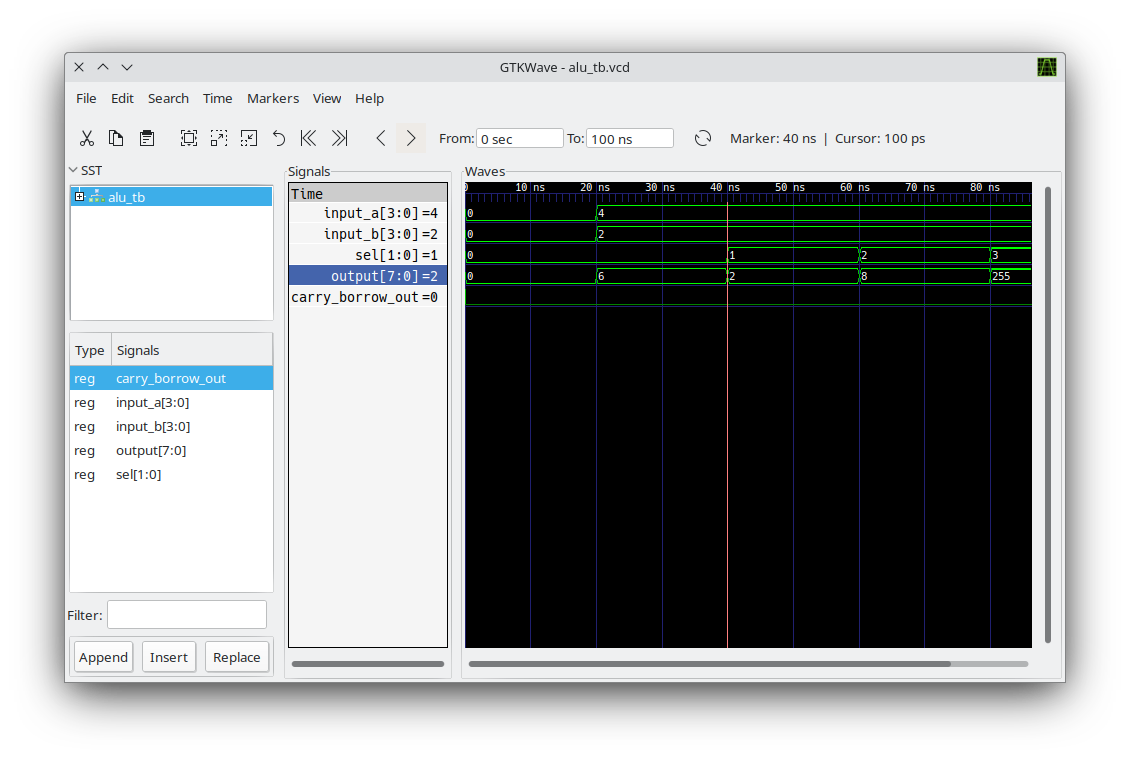
\includegraphics[width=12cm, height=9cm]{./images/alu_vcd}
					\end{center}
			\section{طراحی‌ها}
				\begin{center}
					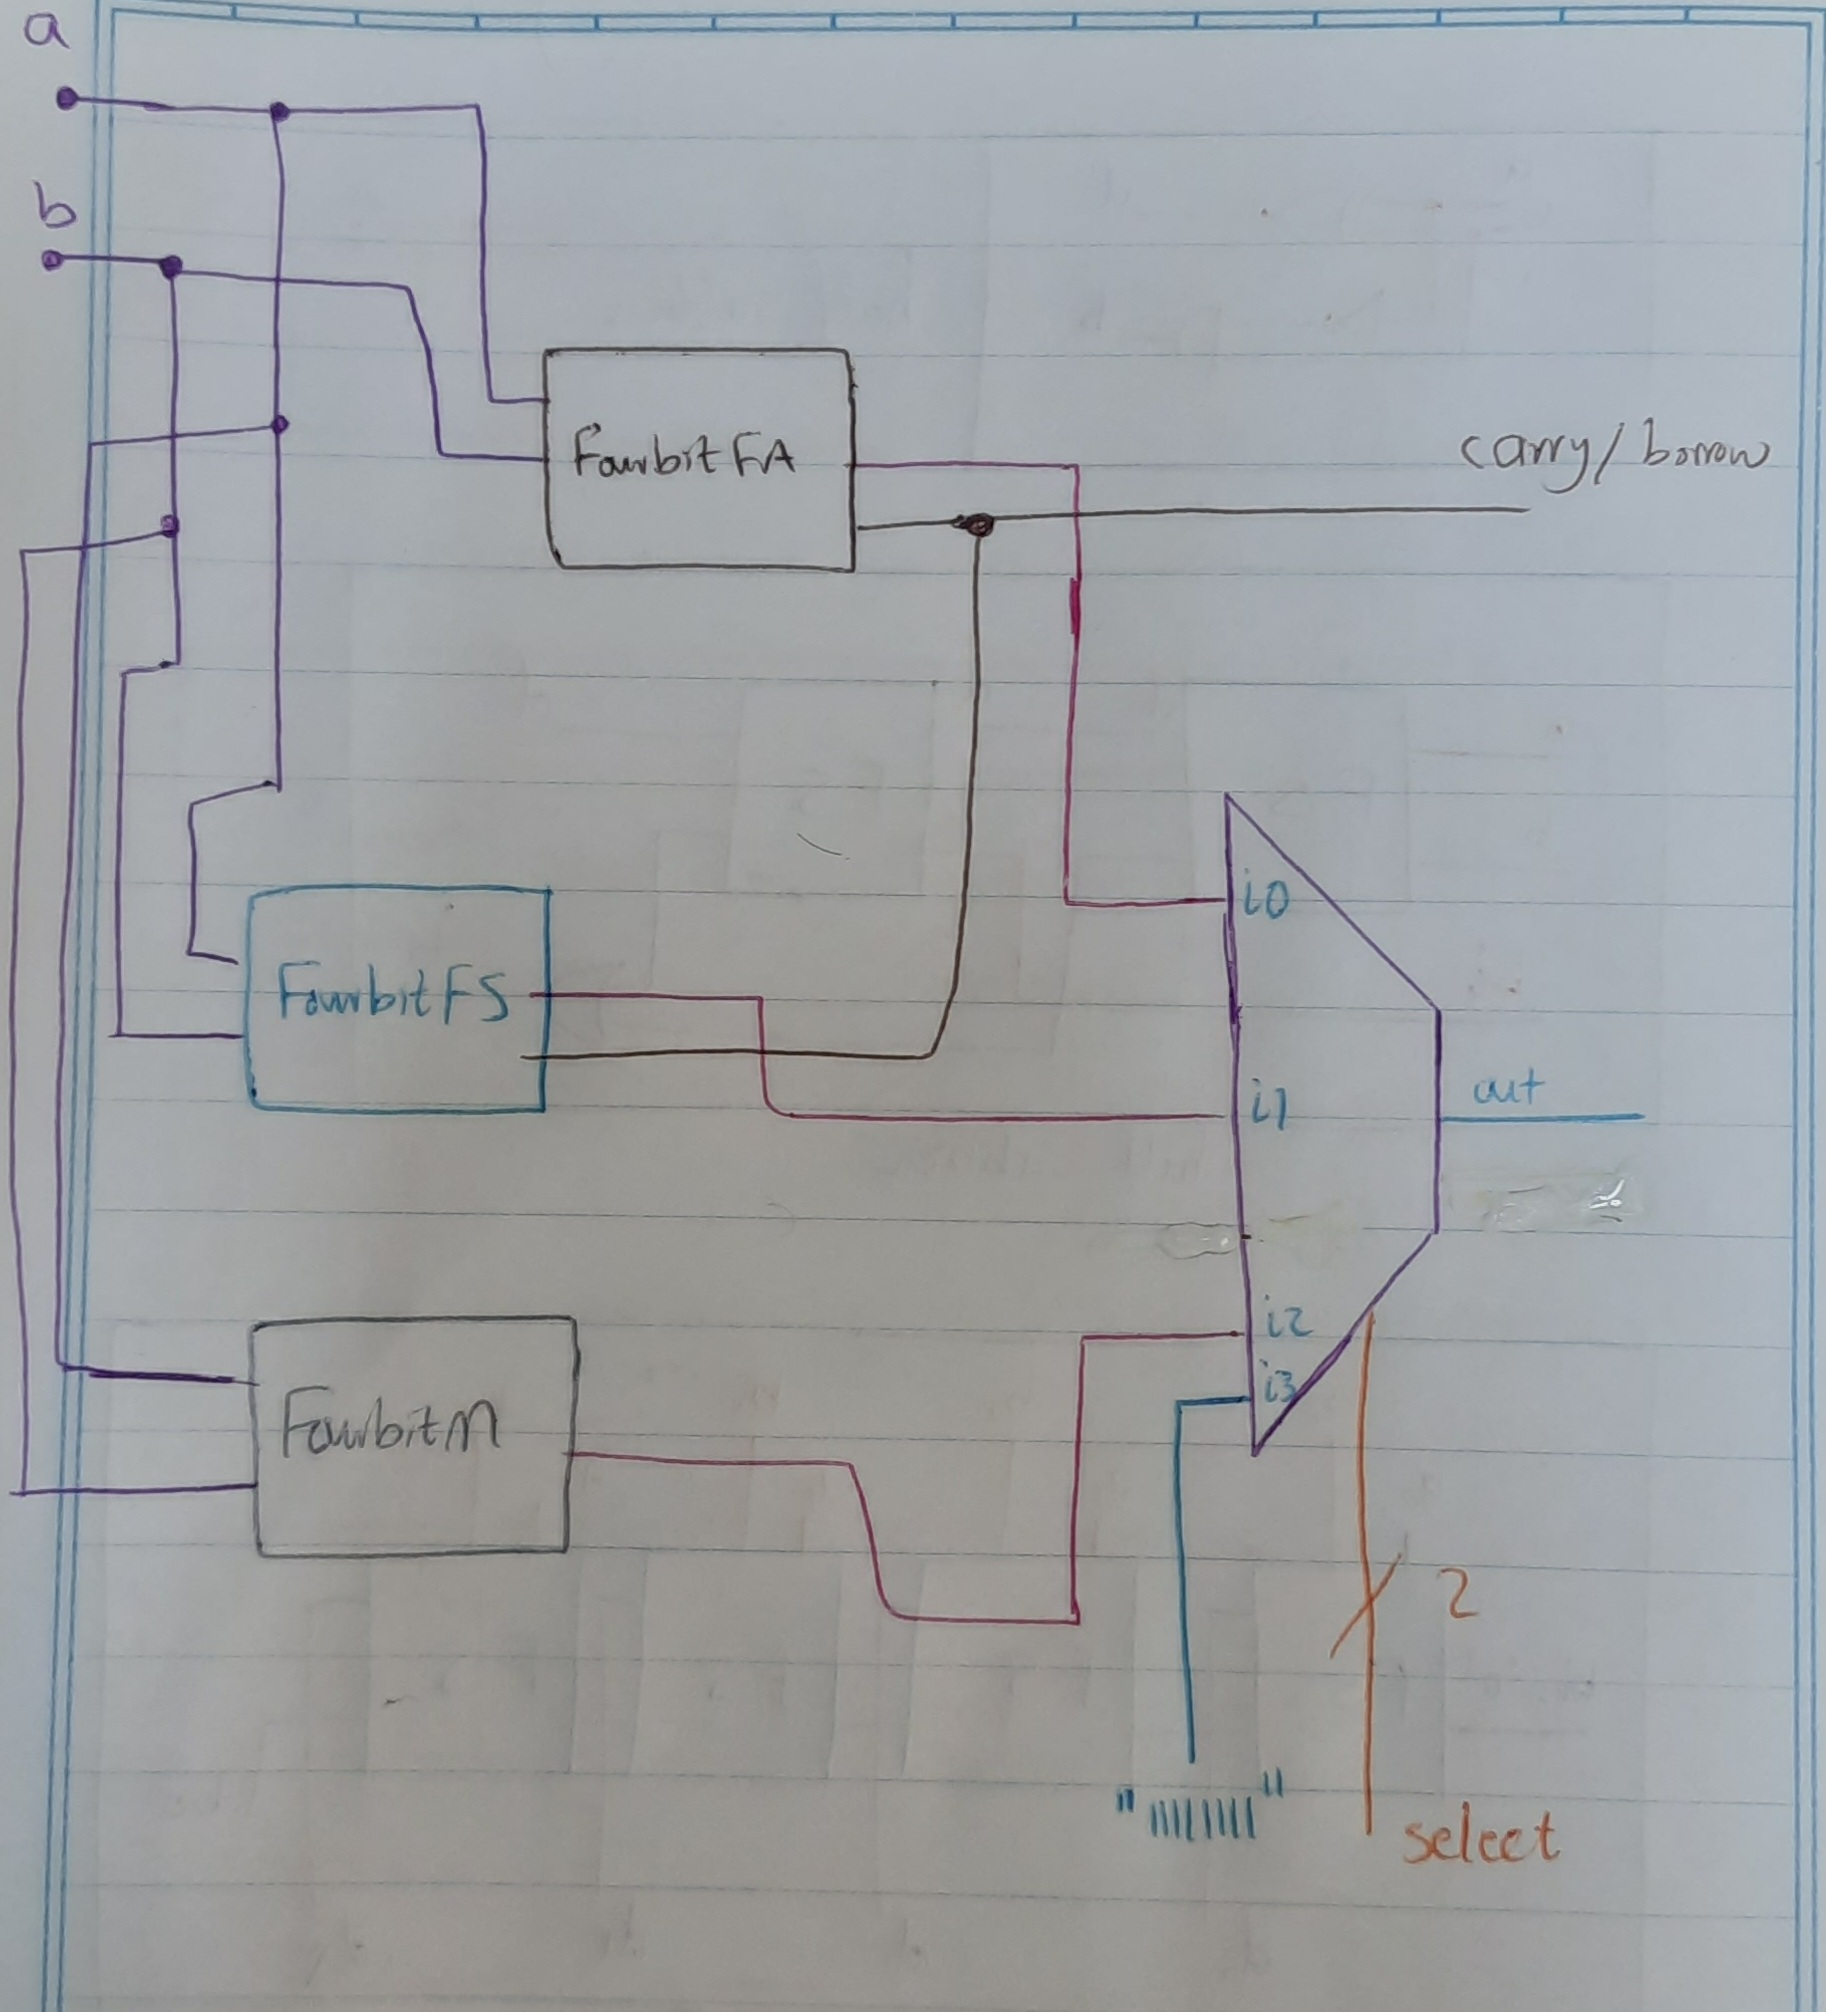
\includegraphics[width=13cm, height=15cm]{./images/alu}
				\end{center}
\end{document}